%                                                                 aa.dem
% AA vers. 9.1, LaTeX class for Astronomy & Astrophysics
% demonstration file
%                                                       (c) ESO 2010
%-----------------------------------------------------------------------
%
%\documentclass[referee]{aa} % for a referee version
%\documentclass[longauth]{aa} % for the long version
%\documentclass[letter]{aa} % for the letters
%\documentclass[bibyear]{aa} % if the references are not structured
%                              according to the author-year natbib style
\documentclass{aa}
%
\usepackage[varg]{txfonts}
\usepackage{graphicx}
\usepackage{float}
\usepackage{natbib}
\bibpunct{(}{)}{;}{a}{}{,}
\usepackage[colorlinks,linkcolor=blue,urlcolor=blue,citecolor=blue]{hyperref}
\usepackage{threeparttablex}
\usepackage{longtable}
\usepackage{lscape}
\usepackage{bm}
\usepackage{verbatim}
\usepackage{makecell}
\usepackage{caption}
\usepackage{subcaption}
\usepackage{multirow}
\usepackage{booktabs}
\usepackage{hyperref}
\usepackage{threeparttable}
\usepackage{colortbl}
\usepackage{xcolor}
\usepackage{booktabs}
\usepackage{graphicx}
\usepackage{txfonts}
%
%
\begin{document}

\title{A Deep X-ray Catalog of Galaxy Groups: Characterizing the Hot Intragroup Medium in COSMOS-Web to $z=3.7$}

\author{Ghassem Gozaliasl\inst{1,2}\thanks{e-mail: ghassem.gozaliasl@aalto.fi}}

\institute{Department of Computer Science, Aalto University, PO Box 15400, 00076, Espoo, Finland\\
\and
Department of Physics, University of Helsinki, Gustaf H\"{a}llstr\"{o}m katu 2, 00560 Helsinki, Finland}

\date{February 25, 2026}

\abstract{
Galaxy groups represent the most abundant environments for galaxies across cosmic time, yet their X-ray properties remain poorly characterized, especially at high redshifts ($z > 1.5$). We present a comprehensive X-ray analysis of 1,678 galaxy groups identified in the COSMOS-Web field using the AMICO algorithm applied to JWST-selected galaxies from the COSMOS2025 catalog. Utilizing deep Chandra and XMM Newton X-ray observations combined with multi-wavelength data from JWST NIRCam, we characterize the hot intragroup medium (IGM) properties including X-ray luminosity, temperature, and entropy out to $z \sim 3.7$. Our analysis reveals significant evolution in X-ray detectability with redshift and halo mass, with implications for understanding AGN feedback efficiency and gas removal processes in groups. We examine the relationship between X-ray detection and optical/NIR group properties, uncovering the diversity of group populations from gas-rich, dynamically relaxed systems to gas-poor systems where feedback may have expelled the hot IGM. By stacking undetected groups, we constrain the average X-ray properties of systems below individual detection thresholds, providing a more complete census of the baryon content and thermal history of the group population. These results bridge X-ray and optical selection methods, establishing the COSMOS-Web group catalog as a unique laboratory for studying group physics and evolution across cosmic time.
}{galaxies: evolution -- galaxies: clusters -- galaxies: groups -- galaxies: high-redshift -- surveys}{}{}{}

\maketitle

%-------------------------------------------------------------------

\section{Introduction}

Galaxy groups represent the most common environment for galaxies in the Universe, hosting the majority of the galaxy population and serving as the building blocks of massive clusters \citep{White1978, Springel2005}. With halo masses spanning $10^{12}$--$10^{14}$~$M_{\odot}$, groups occupy a critical regime where the energy injected by supermassive black hole feedback becomes comparable to the system's binding energy, potentially affecting the entire group volume on megaparsec scales \citep{Popesso2024}. Understanding the properties of the hot intragroup medium (IGM) through X-ray observations provides crucial insights into the thermal history, baryon content, and dynamical state of these systems. The X-ray emission from groups traces the gravitational potential wells of their dark matter halos, offering a direct probe of halo mass and the efficiency of gas heating and cooling processes \citep{Finoguenov2007,George2011}.

Despite their cosmological importance, characterizing the X-ray properties of galaxy groups has remained challenging. The IGM within low-mass halos emits primarily through Bremsstrahlung radiation at temperatures below 1--2~keV, making detection difficult for previous X-ray surveys with limited sensitivity \citep{Ponman1996, Mulchaey2000,Osmond2004,Sun2009,Lovisari2015}. Even with modern facilities like eROSITA, which achieves $\sim$10 times deeper sensitivity than previous all-sky surveys, only a small fraction of the galaxy group population below $10^{14}~M_{\odot}$ is directly detected \citep{Popesso2024}. This shortfall suggests that non-gravitational processes, particularly AGN feedback, may efficiently expel gas beyond the virial radius, reducing hot gas density and X-ray luminosity. Stacking analyses of optically selected groups reveal that undetected systems exhibit lower surface brightness profiles and higher core entropy compared to their detected counterparts at fixed halo mass \citep{Popesso2024,Marini2024}, highlighting the complex interplay between gas physics and halo assembly.

The challenge becomes even more pronounced at high redshifts ($z > 1.5$), where X-ray detections of galaxy groups and clusters become exceedingly rare. While individual massive clusters have been detected in X-rays up to $z \sim 2.0$ \citep{Willis2020}, systematic X-ray surveys of groups at $z > 1.5$ remain limited. Recent work using the AMICO algorithm on COSMOS data has identified 1,269 candidate clusters and groups up to $z = 2$ \citep{Toni2024}. However, direct X-ray detections of groups at $z > 2$ are extremely rare, with most high-redshift systems being identified through optical/NIR overdensities or Sunyaev-Zel'dovich (SZ) signatures. The detection of XLSSC~122 at $z \approx 2.0$ remains one of the few confirmed X-ray-detected clusters at such high redshift \citep{Willis2020}, and only recently has an X-ray-emitting protocluster been detected at $z \approx 5.7$ using combined Chandra and JWST observations \citep{Wang2025}, representing the most distant X-ray detection to date and revealing that substantial ICM heating can occur within the first billion years of cosmic history. At intermediate redshifts ($1.5 < z < 2.5$), spectroscopic surveys have identified massive protostructures \citep{Cucciati2024}, but systematic X-ray characterization remains challenging due to the low surface brightness and extended nature of group-scale emission. This scarcity of high-redshift X-ray detections makes studies of optically/NIR-selected groups particularly valuable, as they enable investigation of the X-ray properties of systems that would otherwise remain undetected in X-ray surveys, extending our understanding of group evolution into the epoch of peak cosmic star formation and structure assembly.

The COSMOS field has been a cornerstone for X-ray studies of galaxy groups and clusters, with previous work identifying 247 X-ray groups at $0.08 \leq z < 1.53$ using XMM-Newton and Chandara observations \citep{Finoguenov2007,George2011,Gozaliasl2019}. These studies revealed fundamental insights into group physics: the importance of precise X-ray center determination using high-resolution Chandra imaging, the relationship between brightest group galaxy (BGG) offsets from X-ray peaks and halo properties, and the substantial scatter ($\sim$0.3~dex) in stellar mass at fixed halo mass \citep{Gozaliasl2016,Gozaliasl2019}. The deep multi-wavelength coverage of COSMOS, combined with extensive spectroscopic and photometric redshift catalogs, enabled robust group identification and characterization across cosmic time, establishing COSMOS as a unique laboratory for studying group evolution.

COSMOS-Web, the largest JWST Cycle~1 programme, extends this legacy into the near-infrared regime, mapping $0.54~\mathrm{deg}^2$ with NIRCam and providing unprecedented depth and resolution for high-redshift galaxy studies \citep{Casey2023}. The COSMOS-Web group catalog, identified using the Adaptive Matched Identifier of Clustered Objects (AMICO) algorithm applied to 389,248 high-quality galaxies from the COSMOS2025 catalog \citep{Shuntov2025}, contains 1678 groups over an effective area of $0.45~\mathrm{deg}^2$ \citep{Toni2025}. This JWST-selected sample, with more than 500 systems possessing spectroscopic confirmations \citep{Khostovan2025}, offers a complementary view to previous X-ray-selected group samples. While X-ray selection naturally favors gas-rich, dynamically relaxed systems, optical/NIR selection captures the full diversity of group populations, including gas-poor systems where feedback may have expelled the hot IGM. This enables studies of the X-ray properties of optically/NIR-identified systems, bridging the gap between selection methods and providing a more complete census of group baryon content.

In this work, we characterize the X-ray emission from COSMOS-Web galaxy groups using a uniform analysis pipeline that applies identical photometric apertures, background subtraction, and calibration choices to every object. Our goals are to (i) quantify the detection rate of diffuse X-ray emission from JWST-identified groups and understand how it differs from X-ray-selected samples, (ii) measure fluxes, luminosities, and mass proxies for individual detections, and (iii) recover ensemble properties via stacking for groups below the individual detection threshold, following the methodology validated in recent stacking and scaling-relation studies of galaxy groups and centrals (e.g.\ \citealt{Anderson2015,PlanckCollaboration2013,Popesso2025,Robson2023,Marini2024}). We analyze both the full COSMOS-Web group sample (CW-All) and a subset of 912 Hickson compact groups (CW-HCG) observed within the COSMOS-Web footprint (Hasinger \& Others in preparation), enabling a controlled comparison between the general group population and compact systems that may represent an earlier stage of group evolution. By combining JWST's deep NIR imaging with the existing COSMOS X-ray data, we probe group X-ray properties across $0.1 \lesssim z \lesssim 3$, spanning the epoch when groups were actively assembling and their baryon content was being shaped by feedback processes.

\section{Data}

\subsection{The COSMOS-Web Survey}

COSMOS-Web is the largest JWST Cycle~1 programme, mapping $0.54~\mathrm{deg}^2$ with NIRCam through the F115W, F150W, F277W, and F444W filters and $0.19~\mathrm{deg}^2$ with MIRI F770W \citep{Casey2023}. The NIRCam imaging reaches $5\sigma$ depths of $26.6$--$27.3$~mag (F115W), $26.9$--$27.7$~mag (F150W), $27.5$--$28.2$~mag (F277W), and $27.5$--$28.2$~mag (F444W) in $0\farcs15$ apertures, providing unprecedented depth and resolution for high-redshift galaxy studies. The survey's deep near-infrared imaging, combined with extensive multi-wavelength coverage from ground-based and space-based facilities, enables robust galaxy identification and characterization across cosmic time.

The COSMOS-Web photometric catalog, derived from deep JWST observations, contains 389,248 high-quality galaxies with precise photometric redshifts ($\sigma_{\rm NMAD} \simeq 0.013$ for sources with F444W $< 25$~mag) and stellar mass estimates \citep{Shuntov2025,Toni2025,Khostovan2025}. This deep, high-quality galaxy sample forms the foundation for group identification using the Adaptive Matched Identifier of Clustered Objects (AMICO) algorithm \citep{Bellagamba2018,Maturi2019}, which has been successfully applied to wide and deep field surveys, including previous applications to COSMOS data up to $z = 2$ \citep{Toni2024}.

\subsection{COSMOS-Web Group Catalog (Toni et al.\ 2025)}

The COSMOS-Web group catalog, presented in \citet{Toni2025}, represents the largest ultra-deep group sample built on JWST observations to date. The catalog was constructed using the Adaptive Matched Identifier of Clustered Objects (AMICO) algorithm \citep{Bellagamba2018,Maturi2019}, which employs a linear optimal matched filter to detect galaxy groups and clusters in photometric redshift catalogs \citep{Toni2025}. AMICO operates by modeling the galaxy density as the sum of signal (cluster/group galaxies) and noise (field galaxies) components. The algorithm generates a three-dimensional amplitude map using position, photometric redshift, and galaxy magnitude, then selects detections at peaks with the highest signal-to-noise ratios. For each candidate, AMICO assigns membership probabilities to galaxies, which are used to compute the apparent richness $\lambda$ (sum of all member probabilities of members brighter than $m_\star + 1.5$ and within $R_{200}$), and the intrinsic richness $\lambda_\star$ (considering only members brighter than $m_\star + 1.5$ and within $R_{200}$), where $m_\star$ is the characteristic magnitude of the luminosity function and $R_{200}$ is the virial radius \citep{Toni2025}.

For the COSMOS-Web application, AMICO was configured with an amplitude-map resolution of $\Delta r = 0.3'$ on the sky plane and $\Delta z = 0.01$ in redshift space, matching the resolution used for the AMICO-COSMOS catalog \citep{Toni2024}. The algorithm used the JWST F150W band magnitude as the single galaxy property, chosen for its good resolution, low background noise, and demonstrated stability in mass-proxy scaling relation calibration at high redshift \citep{Toni2025}. The cluster model incorporated a truncated Navarro--Frenk--White \citep{Navarro1997} profile and a Schechter luminosity function, with the characteristic magnitude $m_\star$ evolving with redshift according to GALEV evolutionary synthesis models for a massive ($\sim 10^{11}~M_{\odot}$) elliptical galaxy formed at $z_f = 8$ with an exponentially declining star formation burst \citep{Toni2025}.

Applying AMICO to the COSMOS-Web galaxy catalog yielded 1678 groups over an effective area of $0.45~\mathrm{deg}^2$ with signal-to-noise ratio $\mathrm{S/N_{nocl}} > 6.0$, extending to redshifts up to $z = 3.7$. The $\mathrm{S/N_{nocl}}$ metric excludes shots noise from cluster/group members in the amplitude variance, providing a more stable redshift dependence of sample purity compared to the standard $\mathrm{S/N}$ \citep{Toni2025}. The catalog achieves a purity level of $\sim$77\% for the full sample, with approximately 670 groups detected at a purity of 90\%. More than 500 systems possess spectroscopic confirmations \citep{Khostovan2025}, providing robust redshift measurements for a significant fraction of the sample.

Brightest group galaxies (BGGs) in the catalog were selected using a hybrid scheme that evaluates both stellar mass and F150W luminosity within 250--500~kpc apertures, ensuring robust identification of the central galaxies. The catalog provides celestial coordinates, redshifts (both photometric and spectroscopic where available), richness estimates ($\lambda_\star$), and BGG properties, enabling comprehensive studies of group properties and galaxy evolution in different environments.

For the present X-ray analysis, we utilize the full COSMOS-Web group sample (hereafter CW-All), corresponding to all 1678 systems from the \citet{Toni2025} catalog. This sample spans $0.1 \lesssim z \lesssim 3.7$, covering nearly 12~Gyr of cosmic history and enabling studies of group X-ray properties from the least rich population of groups to the formation of the most massive clusters.

\subsection{Hickson Compact Groups (Hasinger et al.\ in preparation)}

In addition to the full COSMOS-Web group catalog, we analyze a complementary sample of 912 Hickson compact groups (hereafter CW-HCG) observed within the COSMOS-Web footprint (Hasinger \& Others in preparation). Hickson compact groups were originally defined by \citet{Hickson1982} based on specific selection criteria: (1) containing at least four galaxies within a magnitude range of 3~mag from the brightest member, (2) having a high surface density such that the angular diameter of the smallest circle containing the group centers is less than three times the diameter of the largest galaxy, and (3) being isolated from other galaxies of comparable brightness. These criteria select systems with typically 4--5 galaxies in a compact configuration, high surface density, and low velocity dispersion.

The original Hickson catalog identified 100 compact groups in the local universe based on visual inspection of photographic plates, with a median rest-frame surface brightness in the R band of $\mu_R \sim 26.5$~mag~arcsec$^{-2}$ \citep{Hickson1982}. Subsequent studies have shown that compact groups represent dense, dynamically evolving systems where galaxies are in close proximity and may be undergoing active interactions and mergers \citep{MendesDeOliveira1994}. These systems are thought to represent an earlier stage of group evolution or a distinct class of dense groups that may eventually merge to form a single galaxy.

The CW-HCG sample provides a controlled comparison to the general group population, enabling investigation of whether compact groups exhibit different X-ray properties compared to the broader group population. This comparison is particularly valuable for understanding the role of group compactness and dynamical state in shaping the hot intragroup medium, as compact groups may represent systems in earlier stages of virialization or undergoing more active assembly processes. The high surface density and close galaxy separations in compact groups may lead to enhanced tidal interactions and gas stripping, potentially affecting the X-ray emission properties of the intragroup medium.

\subsection{X-ray Data and Observations}

The X-ray data used in this work are based on the combined Chandra and XMM-Newton observations of the COSMOS field, following the methodology described in \citet{Gozaliasl2019}. The XMM-Newton Wide-Field Survey in the COSMOS field \citep{Hasinger2007} provides deep X-ray coverage of the full $2~\mathrm{deg}^2$ COSMOS field, with 55 XMM-Newton pointings totaling approximately 1.5~Ms of exposure time and an average vignetting-corrected depth of 40~ks. The Chandra COSMOS-Legacy Survey \citep{Elvis2009,Civano2016,Marchesi2016} provides high-resolution imaging across the full COSMOS field, complementing the XMM-Newton observations that were used in earlier group catalogs \citep{Finoguenov2007,George2011}. The revised X-ray catalog of extended sources in COSMOS was obtained by co-adding all available Chandra and XMM-Newton data in the field, reaching an X-ray flux limit of $3 \times 10^{-16}~\mathrm{erg~cm^{-2}~s^{-1}}$ in the $0.5$--$2.0$~keV band \citep{Gozaliasl2019}.

On spatial scales of 32--128$''$ used for group detection, the combined Chandra data adds approximately 30\% to the existing XMM-Newton exposure (or 14\% in sensitivity) on average. However, the primary advantage of incorporating Chandra data lies in the improved precision of X-ray center determination for extended sources. By utilizing smaller-scale emission detected by Chandra ($16''$ scales), the statistical uncertainty on centering was reduced from 15$''$ in previous XMM-only catalogs to 5$''$ \citep{Gozaliasl2019}. This improved centering precision is crucial for accurately measuring the offset between brightest group galaxies and X-ray peaks, and for distinguishing between central dominant and offset BGGs.

The X-ray maps used in this analysis are distributed together with their $1\sigma$ uncertainty images. The images have $4''$ pixels, conservative masking of bright point sources, and homogenized exposure weighting that allows direct aperture photometry without further rescaling. The primary maps store background-subtracted count rates in counts~s$^{-1}$~pixel$^{-1}$, while the companion uncertainty maps record the formal errors on the same scale. Residual soft-proton flares were filtered during the map construction, leaving approximately Poissonian noise within the apertures and annuli defined in Section~\ref{sec:analysis}. For this work, we use the full X-ray map to ensure consistent analysis across all redshift ranges and to avoid discontinuities in the stacking analysis that can arise from switching between masked and unmasked maps at different redshifts.

Figure~\ref{fig:xray_map} shows the full COSMOS X-ray map in the 0.5--2.0~keV band, covering the $2~\mathrm{deg}^2$ COSMOS field. The map combines Chandra and XMM-Newton observations, providing deep X-ray coverage used for the group analysis. Bright point sources and extended emission from clusters and groups are visible throughout the field. The inset illustrates the aperture and background geometry for a detected group (Group 1, CW-All ID=1.0, SNR=28.2, $z = 0.710$): the source aperture (green circle, here equal to $R_{500}$), the background annulus used for background determination (blue dashed $=$ inner radius, orange dashed $=$ outer radius, corresponding to $2\,R_{500}$--$3\,R_{500}$ for this object), and the $R_{200}$ circle (purple). The red cross marks the catalog centre (optical/NIR group centre from AMICO); the green plus sign marks the X-ray peak (flux-weighted centroid used for the refined photometry of detections); the gold star marks the brightest group galaxy (BGG). This layout shows how the background is measured outside the source aperture and how catalog centre, X-ray peak, and BGG can be compared (see Section~\ref{sec:background}).

Figure~\ref{fig:group1_rgb} presents a composite JWST NIRCam RGB image of Group~1 (CW-All ID=1.0, $z = 0.710$, SNR=28.2) with the Chandra+XMM-Newton X-ray emission overlaid in purple, illustrating the spatial coincidence of the hot intragroup medium with the galaxy overdensity. The diffuse X-ray glow traces the gravitational potential well of the group halo, while the JWST imaging reveals the member galaxies and their morphologies in exquisite detail. This system represents the highest-significance X-ray detection in our sample and serves as a showcase example of the multi-wavelength data available for COSMOS-Web groups.

Figure~\ref{fig:redshift_dist} presents the redshift distribution of both catalogs, showing that the CW-All sample spans $0.08 \lesssim z \lesssim 3.70$ with a median redshift of $z \approx 1.1$, while the CW-HCG sample covers $0.12 \lesssim z \lesssim 3.83$ with a median redshift of $z \approx 0.97$. The redshift distributions reveal that both samples peak at $z \sim 1$--1.5, corresponding to the epoch of peak cosmic star formation and structure assembly. The CW-HCG sample shows a slightly lower median redshift, consistent with the expectation that compact groups may represent earlier stages of group evolution or preferentially form at lower redshifts where galaxy interactions are more common.

\section{Analysis methodology}
\label{sec:analysis}

Every object in both catalogs was processed through the same sequence of observational steps so that differences between CW-All and CW-HCG reflect astrophysics rather than analysis choices. The pipeline uses adaptive apertures, a redshift-binned median background technique, adaptive sigma clipping in the background annulus, and a two-pass scheme: an initial pass with a fixed physical aperture for detection, followed by refinement of detected sources using true $R_{500}$ and $R_{200}$ from scaling relations, adaptive background annuli, and X-ray peak centering.

\noindent\textbf{Observables and conventions.} We work in the rest-frame 0.5--2.0~keV band. The primary observable reported for each group is the rest-frame X-ray luminosity $L_{\rm X}$. For sources above the detection threshold we report the measured $L_{\rm X}$; for the remainder we report 95\% upper limits. We also derive intragroup medium temperature $T$, halo mass $M_{\rm A}$, and characteristic radii $R_{200}$ and $R_{500}$ from scaling relations tied to $L_{\rm X}$. We give first the scaling relations and the conversion from count rate to flux and $L_{\rm X}$ (\S\ref{sec:scaling}--\ref{sec:kcorr}), then the measurement flow (coverage, apertures, background, detection) that yields net counts and thus flux and $L_{\rm X}$.

\subsection{Scaling relations for temperature and mass}
\label{sec:scaling}

For the majority of sources we do not have direct temperature measurements; we therefore estimate the intragroup medium temperature from the rest-frame soft-band luminosity. We use the bias-corrected $L_{\rm X}$--$T_{\rm X}$ relation from \citet{Kettula2015} (CFHTLenS weak lensing calibrated), which can be written
\begin{equation}
T_{\rm X} = T_0 \left( \frac{L_{\rm X}\, E(z)^{-1}/L_0}{A_{\rm LT}} \right)^{1/\alpha_{\rm LT}},
\label{eq:TL}
\end{equation}
with $T_0 = 5$~keV, $L_0 = 10^{44}$~erg~s$^{-1}$, $A_{\rm LT} = 1.51$, and $\alpha_{\rm LT} = 2.52$ (so $T_{\rm X} \propto (L_{\rm X}\, E(z)^{-1})^{1/2.52}$). For groups with measured temperatures this relation is not used; the measured $T$ is adopted. We assign a fractional uncertainty of 50\% to the luminosity-based temperature estimate to reflect the intrinsic scatter of the relation and the lack of multi-band constraints.

Halo masses are derived from two relations that we keep self-consistent. The primary relation is the weak-lensing calibrated mass--luminosity relation from \citet{Leauthaud2010}, from which we model and evolution of the mass--luminosity relation for X-ray groups in the COSMOS field using weak lensing. In the form used here,
\begin{equation}
M_{200}\, E(z) = A_{\rm ML} \left(\frac{L_{\rm X}\, E(z)^{-1}}{L_{{\rm X},0}}\right)^{\alpha_{\rm ML}} M_0,
\label{eq:ML}
\end{equation}
with $\alpha_{\rm ML} = 0.64$, $A_{\rm ML} = 1.17$, $L_{{\rm X},0} = 5.01 \times 10^{42}$~erg~s$^{-1}$, and $M_0 = 5.01 \times 10^{13}~M_{\odot}$. Rearranging, $M_{200} = A_{\rm ML}\,(L_{\rm X}\,E(z)^{-1}/L_{{\rm X},0})^{\alpha_{\rm ML}} M_0/E(z)$. We adopt an intrinsic scatter of $\sim 0.30$~dex. This gives the direct $L_{\rm X} \to M_{200}$ mass estimate.

For the conversion from temperature to mass we use an $M$--$T$ relation that is derived from the same \citet{Leauthaud2010} $M$--$L_{\rm X}$ relation and the \citet{Kettula2015} $L_{\rm X}$--$T$ relation above, so that the chain $L_{\rm X} \to T \to M$ yields the same $M$ as $L_{\rm X} \to M$ directly. The combined slopes are $\alpha = \alpha_{\rm ML}\,\alpha_{\rm LT} = 0.64 \times 2.52 \approx 1.61$, and the $E(z)$ dependence follows from the Leauthaud relation. The resulting $M_{500}$--$T$ relation is
\begin{equation}
M_{500} = A_{500} \left(\frac{T}{T_0}\right)^{\alpha} E(z)^{-1} \times 10^{14}~M_{\odot},
\label{eq:MT}
\end{equation}
with $T_0 = 5$~keV and normalization $A_{500} \approx 7.35$ set by matching $M_{500}$ to the $M$--$L_{\rm X}$ prediction at a reference temperature. We convert to $M_{200}$ via $M_{200} = 1.4\,M_{500}$, corresponding to a Navarro--Frenk--White \citep{Navarro1997} concentration $c \approx 4$.

Characteristic radii are computed as
\begin{equation}
R_{\Delta} = \left[\frac{3 M_{\Delta}}{4\pi \Delta \rho_c(z)}\right]^{1/3},
\label{eq:RDelta}
\end{equation}
with $\Delta = 200, 500$ and $\rho_c(z)$ the critical density at redshift $z$. Reported mass uncertainties incorporate measurement errors and the adopted intrinsic scatters.

\subsection{Spectral model and flux conversion}
\label{sec:flux}

Net count rates divide by the effective exposure time implicit in the count-rate map. We then translate count rate to energy flux using the same MOS1+MOS2 energy-conversion factor that was adopted when constructing the COSMOS mosaic. The calibration assumes a $\Gamma = 2.0$ spectrum with Galactic absorption $N_{\rm H} = 2.5 \times 10^{20}$~cm$^{-2}$. The resulting factor,
\begin{equation}
C_{\rm XR} = 1.082 \times 10^{-11}~\mathrm{erg~cm^{-2}~count^{-1}},
\label{eq:CXR}
\end{equation}
matches the value supplied with the mosaic products and is implemented via the \texttt{xray.count\_rate\_to\_flux} configuration parameter. The true conversion varies with the assumed spectral shape and spatial weighting across the detectors; we therefore propagate a systematic uncertainty of $\pm10\%$ to reflect plausible variations in photon index and $N_{\rm H}$, and expose the conversion factor in the analysis configuration so that alternative calibrations can be tested.

\subsection{Luminosity calculation and K-correction}
\label{sec:kcorr}

The rest-frame 0.5--2.0~keV luminosity $L_{\rm X}$ (the primary observable reported for each group; see \S\ref{sec:detection}) is computed from the energy flux via
\begin{equation}
L_{\rm X} = 4\pi\, D_{\rm L}^2\, F_{\rm X}\, K(z, T),
\label{eq:LX}
\end{equation}
where $D_{\rm L}$ is the luminosity distance. The $K$-correction $K(z, T)$ is computed from the same APEC spectrum used for the flux conversion, evaluated at the object's redshift \citep{Finoguenov2007,Leauthaud2010}. In practice, the temperature dependence of $K$ in this band remains modest ($< 10\%$) for $0.5 \lesssim kT \lesssim 3$~keV; we therefore evaluate $K$ at $kT = 1$~keV but propagate a 10\% systematic uncertainty on the luminosity to reflect the plausible range of temperatures.

\subsection{Coverage and cosmological distances}
\label{sec:coverage}

Sky coordinates supplied by the catalogs were converted to pixel positions on the 0.5--2.0~keV mosaic using the FITS World Coordinate System (WCS). Sources falling on masked or non-finite pixels (typically chip gaps or edge artefacts) were excluded; in practice every catalogued group remained within the usable region. Angular-diameter distances, required to convert between physical and angular scale, were computed with a Planck-2018 flat $\Lambda$CDM cosmology \citep{Aghanim2020} ($H_0 = 67.4$~km~s$^{-1}$~Mpc$^{-1}$, $\Omega_{\rm m} = 0.315$).

\subsection{Aperture definition, adaptive radius, and extent handling}
\label{sec:aperture}

The baseline source aperture is a physical radius of 300~kpc centred on each group. For a given redshift $z$ the angular radius is
\begin{equation}
\theta_{\rm src} = \frac{300~\mathrm{kpc}}{D_{\rm A}(z)},
\label{eq:theta}
\end{equation}
where $D_{\rm A}$ is the angular-diameter distance; the result is converted to arcseconds. Minimum and maximum angular sizes of $5''$ and $120''$ prevent unphysical apertures for very nearby or distant sources.

The workflow uses two passes. First pass: photometry is performed for all groups with the 300~kpc aperture and a fixed physical background annulus (see \S\ref{sec:background}) to derive net counts, SNR, fluxes, luminosities, and mass proxies. Detection is based on SNR~$\geq 2.0$ (see \S\ref{sec:detection}). Second pass (refinement of detections): for each detected source we compute $R_{500}$ and $R_{200}$ from the scaling relations (see \S\ref{sec:scaling}). The source aperture is then set to $R_{500}$ when available, otherwise to $R_{200}$, converted to arcseconds and clipped to the same $5''$--$120''$ range. The background annulus for detected groups is switched to an adaptive, $R_{500}$-scaled annulus (inner $= 2\,R_{500}$, outer $= 3\,R_{500}$) to reduce contamination from extended emission or nearby sources. We also recentre the measurement on the X-ray peak by finding the flux-weighted centroid (or local peak) within $R_{500}$ or $R_{200}$; photometry is then re-run only for detected groups with these updated apertures, centres, and background annuli. Non-detected groups retain the first-pass 300~kpc aperture and fixed background.

Whenever a catalog provides an intrinsic extent estimate (e.g.\ optical or X-ray size), we convert the supplied value to arcseconds according to the stated units (arcsec, arcmin, kpc, or detector pixels), apply an optional scale factor, and clip to the same angular bounds. When extent application is set to ``detected'', only detected sources with a valid extent have their aperture replaced by the catalogued extent (subject to the same $5''$--$120''$ limits) before the refined photometry run. This adaptive radius and extent handling keeps a single, well-defined detection step while allowing physically motivated apertures and centres for the reported fluxes and luminosities of detections.

\subsection{Background determination and redshift-binned median}
\label{sec:background}

Background is estimated from a concentric annulus around each source. First pass and non-detected groups: the annulus spans 450--750~kpc in physical scale, converted to angular size at the source redshift and forced to lie at least $1''$ beyond the source aperture. Detected groups (refined pass): the annulus is adaptive, inner radius $= 2\,R_{500}$ and outer radius $= 3\,R_{500}$, again with a $1''$ gap outside the source aperture. The inset in Figure~\ref{fig:xray_map} illustrates this geometry for a detected group: the source aperture (green circle, $R_{500}$), the background annulus (blue and orange dashed circles), and the distinction between the catalog centre (red X), the X-ray peak (green plus) used for refined photometry, and the BGG (gold star).

Before integrating the annulus we (i) build a contamination mask that excludes pixels lying inside any other group's source aperture, so that projected neighbours do not bias the background, and (ii) apply adaptive sigma clipping within the annulus. Sigma clipping is iterative: pixels deviating by more than a threshold from the median are removed. To avoid over-clipping when contamination is non-uniform (e.g.\ residual point-source wings affecting only part of the annulus), we try a sequence of thresholds (e.g.\ $2.5\sigma$, $2.0\sigma$, $1.5\sigma$) and retain the least aggressive threshold for which at least 5\% of the annulus pixels survive; if no threshold meets this criterion, we use the raw annulus. This adaptive clipping suppresses bright outliers while preserving a stable background estimate.

In addition to the per-source annulus background, we compute a redshift-binned median background for quality control and comparison. For each group we take the annulus-derived background surface brightness (counts per pixel) of all groups in a sliding redshift window $z \pm \Delta z$ (default $\Delta z = 0.05$). If fewer than a minimum number of groups (default 5) fall in the window, the window is expanded (up to $2\,\Delta z$). The median of these surface brightness values is converted to a background count estimate for the group's aperture area. Net counts and SNR derived from this binned-median background are stored alongside the annulus-based values; the primary fluxes and luminosities reported in this work use the annulus-based background, with the binned-median results used as a cross-check.

\subsection{Background subtraction and error propagation}
\label{sec:errprop}

Circular apertures and annuli were evaluated on the exposure-corrected count-rate map and its uncertainty image. Source counts are the sum of pixel values within the source aperture (with partial pixels weighted by the aperture mask). Background counts are the sum over the annulus after contamination masking and sigma clipping, scaled to the source aperture area so that the background contribution is correct for each source's angular size. The per-pixel error map is squared before integration; the square root of the summed variance gives the uncertainty on the source and background sums. Net counts are $C_{\rm net} = C_{\rm src} - C_{\rm bkg,scaled}$, and the net uncertainty is $\sigma_{\rm net} = \sqrt{\sigma_{\rm src}^2 + \sigma_{\rm bkg,scaled}^2}$. For each aperture we record the fraction of unmasked pixels; sources with coverage below 50\% are flagged and excluded from flux and mass estimates.

\subsection{Detection significance threshold}
\label{sec:detection}

We tested detection thresholds of SNR~$\geq 1.5$, $2.0$, $2.5$, and $3.0$ using a dedicated sweep over the full pipeline. The resulting catalogues show qualitatively identical trends; higher thresholds yield progressively fewer, brighter detections. We adopt SNR~$\geq 2.0$ as the baseline because it balances robustness against false positives with sufficient statistics for catalogue-level and stacking comparisons; the corresponding single-trial Gaussian false-alarm probability is 2.3\%.

Detection significance is characterised by the signal-to-noise ratio,
\begin{equation}
\mathrm{SNR} = \frac{C_{\rm net}}{\sigma_{\rm net}},
\label{eq:SNR}
\end{equation}
where $C_{\rm net}$ and $\sigma_{\rm net}$ are the background-subtracted counts and their uncertainty. Upper limits for non-detections are derived as $C_{\rm net} + 1.645\,\sigma_{\rm net}$ (95\% confidence) and subsequently propagated to fluxes and luminosities. For sources that fall below the detection threshold we still report X-ray constraints by evaluating
\begin{equation}
C_{\rm UL} = \begin{cases}
\mathrm{PoissonPPF}(0.95,\,\sigma_{\rm bkg}^2) & \text{if } C_{\rm net} \leq 0, \\
C_{\rm net} + 1.645\,\sigma_{\rm net} & \text{otherwise},
\end{cases}
\label{eq:UL}
\end{equation}
where $\sigma_{\rm bkg}$ is the background standard deviation. This hybrid Bayesian scheme recovers the appropriate Poisson upper limit for apertures dominated by background noise while reducing to the Gaussian form for higher-count measurements.

To identify potentially problematic non-detections that may arise from aperture contamination or measurement systematics, we compare the upper-limit flux distribution against the detected source distribution. We flag non-detections whose 95\% upper-limit flux falls below the first quartile (Q1) of the detected flux distribution, as these sources likely represent measurement artefacts rather than genuinely faint intragroup emission. Figure~\ref{fig:upper_limits} visualizes this diagnostic: the left panel compares the flux distributions of detected sources, all upper limits, and flagged upper limits, while the right panel shows the redshift distribution of flagged versus unflagged non-detections. The baseline stacks include all groups, but we track the flagged subset separately and confirm that masking them changes the stacked fluxes by less than the statistical uncertainties.

\section{X-ray analysis results}

\subsection{X-ray luminosity and the $L_{\rm X}$--redshift plane}
\label{sec:LX_z}

The primary diagnostic quantity we report for each group is the rest-frame 0.5--2.0~keV X-ray luminosity $L_{\rm X}$. For detections (SNR~$\geq 2.0$) we report the measured $L_{\rm X}$; for non-detections we report 95\% upper limits propagated from the count-rate upper limits (see above). Figure~\ref{fig:LX_z} shows the $L_{\rm X}$--redshift plane for both CW-All and CW-HCG. Individual detections (large open circles) populate the upper envelope of the distribution; non-detections appear as grey points (95\% upper limits), with blue points highlighting those whose upper limit falls below the first quartile of the detected flux distribution (flagged for quality control). Orange squares indicate the stacked median luminosities in each redshift bin (see \S\ref{sec:stacking}). This figure is the central diagnostic for the remainder of the paper: it illustrates the detection rate as a function of redshift, the separation between detections and upper limits, and the consistency of stacked luminosities with the envelope of individual detections. The detailed conversion from net counts to flux and from flux to $L_{\rm X}$ is given in \S\ref{sec:flux} and \S\ref{sec:kcorr}.

\subsection{Halo mass and the $M_{200}$--redshift plane}

To complement the $L_{\rm X}$--redshift plane, Figure~\ref{fig:M200_z} shows halo mass $M_{200}^{L_{\rm X}}$ as a function of redshift for individually detected groups in the CW-All and CW-HCG samples, derived from the weak-lensing calibrated $M$--$L_{\rm X}$ scaling relation of \citet{Leauthaud2010}. This panel highlights the mass range and redshift leverage of our X-ray-detected systems and illustrates that both samples predominantly probe group-scale halos across the full redshift span of the survey.

\subsection{Stacking procedure}
\label{sec:stacking}

To characterise populations that fall below the single-object detection threshold we perform stacking in redshift bins. For each bin we extract postage-stamp cutouts centred on the catalogued positions, with a radius three times the source aperture to encapsulate the background annulus. Each cutout is background-subtracted locally using annuli scaled by factors of 1.5 and 3.0 relative to the source aperture, mirroring the single-object measurement. The background-subtracted counts are then combined on a source-by-source basis. We compute both the mean and median of the surviving aperture sums, applying a sigma-clipping threshold of $2\sigma$ to remove outliers (e.g.\ residual point sources). Bootstrap resampling with 1000 iterations yields the uncertainty on the adopted central estimator. Stacked count rates, fluxes, luminosities, and mass proxies are derived in the same fashion as for individual detections, using the median redshift of each bin. Bins containing fewer than five sources are flagged as low fidelity, although for completeness we still report the measured values with appropriate cautions.

\subsection{Detection results}

Both catalogs show modest detection rates, reflecting the low surface brightness of intragroup gas at the survey depths. Table~\ref{tab:detection} summarises the key detection statistics.

The detection fractions of $\sim 30$--33~per~cent highlight the improved sensitivity achieved with the refined redshift measurements and optimized analysis pipeline. Detected systems in both samples cluster around $z \sim 1$ and exhibit median luminosities near $10^{42.9}$~erg~s$^{-1}$, consistent with group-scale halos hosting hot atmospheres. The CW-HCG sample shows a slightly higher detection rate (33.4\%) compared to CW-All (29.6\%), which may reflect the enhanced surface brightness of compact group cores, though both samples probe similar luminosity regimes.

Figure~\ref{fig:LX_z} presents the $L_{\rm X}$--redshift primary diagnostic analysis. The $L_{\rm X}$--redshift plane (Figure~\ref{fig:LX_z}, introduced in \S\ref{sec:LX_z}) summarises detections and upper limits for both samples, with stacked medians from Section~\ref{sec:stacking} over-plotted.

\subsection{Stacking analysis}

Given the prevalence of non-detections, stacking was crucial to recovering ensemble X-ray properties. The procedure described in Section~\ref{sec:stacking} delivered high-SNR composite detections in all five redshift bins for both catalogs. Table~\ref{tab:stacking_all} lists the CW-All ensemble measurements, while Table~\ref{tab:stacking_hcg} reports the CW-HCG results.

Both samples yield significant stacked detections in every bin, validating the presence of diffuse intragroup gas despite the low individual detection rate. Figure~\ref{fig:stacking} summarises the stacked rest-frame luminosities, observed-frame fluxes, SNR, and $M_{200}^{L_{\rm X}}$ as a function of redshift for both catalogs, and directly compares stacks built from all groups in each bin (solid curves) to stacks restricted to individually detected systems (dashed). The close agreement between the all-groups and detections-only curves at $z \lesssim 2$ indicates that the stacked signals are representative of the full group population rather than being driven solely by a small number of bright detections; differences in the highest-redshift bins mainly reflect the limited number of compact groups and the increasing prevalence of massive halos in the CW-All sample.

\subsection{Summary}

Using a uniform X-ray analysis pipeline with a SNR~$\geq 2.0$ detection threshold, we detect X-ray emission from 305 CW-HCG groups (33.4\%) and 497 CW-All groups (29.6\%). Detected systems exhibit median luminosities of $10^{42.9}$~erg~s$^{-1}$ and temperatures around 1.3--1.4~keV, indicative of group-scale hot atmospheres. Stacking across five redshift bins yields high-significance detections for both samples, revealing steadily increasing luminosities with redshift and halo masses of order $\log_{10}(M_{200}/M_{\odot}) \approx 12$. The similar stacked luminosities of the CW-All and CW-HCG samples up to $z \sim 2$ suggest that compact group cores do not necessarily enhance the global X-ray output relative to the general group population when averaged over large samples. At higher redshift, the CW-All sample exhibits higher SNR and luminosities, likely reflecting the inclusion of more massive halos identified via the COSMOS-Web selection. The moderate temperatures ($T \sim 1.3$--1.4~keV) inferred for individual detections align with expectations for group-scale masses. All X-ray catalogs (\texttt{xray\_catalog.fits}) include source-by-source photometry, detection flags, and physical properties and are ready for further scientific exploitation.

%-------------------------------------------------------------------

\begin{appendix}

\section{Radial surface-brightness stacking and PSF tests}

\subsection{Radial surface-brightness profiles}

We measure stacked X-ray surface-brightness profiles around COSMOS-Web galaxy groups using the combined XMM-Newton$+$Chandra 0.5--2~keV mosaic. For each group, we extract a square X-ray cutout centred on the group position and convert angular to physical scales using our fiducial Planck 2018 cosmology ($H_0 = 67.4$~km~s$^{-1}$~Mpc$^{-1}$, $\Omega_{\rm m} = 0.315$, $\Omega_\Lambda = 0.685$). This procedure is conceptually similar to large-sample stacking analyses of locally brightest galaxies and optically selected groups in ROSAT, eROSITA, and Planck data (e.g.\ \citealt{Anderson2015,PlanckCollaboration2013,Popesso2025}), but applied here in redshift bins rather than halo-mass bins.

Within each redshift bin all groups share a common set of physical radius bins $[r_i]$ (typically $\sim$10--15~kpc wide, extending to $r \sim 200$--300~kpc). For each cutout we compute the distance $R$ of every pixel from the group centre in kpc, and accumulate, in each annulus $i$, the total counts and number of valid pixels (excluding masked pixels and NaNs). The mean surface brightness in annulus $i$ for group $g$ is
\begin{equation}
S_{g,i} = \frac{\sum_{p \in i} C_p}{N_{p,i}},
\label{eq:Sgi}
\end{equation}
where $C_p$ is the counts in pixel $p$ and $N_{p,i}$ is the number of good pixels in that annulus. This yields one one-dimensional surface-brightness profile $S_{g,i}$ per group.

\subsection{Weighted stacking of groups}

Within each redshift bin we stack the individual profiles into a single mean profile, while allowing for different detection significance and data quality through per-group weights. For each group we match to the X-ray catalog and construct a simple weight
\begin{equation}
w_g = \frac{1}{1 + f_g},
\label{eq:wg}
\end{equation}
where $f_g = 0$ for robust X-ray detections and $f_g = 1$ for non-detections or flagged sources (e.g.\ suspected false positives or projected contaminants, when available). Thus clean detections receive $w_g = 1$ and non-detections or flagged non-detected systems receive $w_g = 0.5$, down-weighting ambiguous or non-detected systems without discarding them.

In each radial bin $i$ we compute the weighted mean surface brightness
\begin{equation}
\bar{S}_i = \frac{\sum_g w_g\, S_{g,i}}{\sum_g w_g},
\label{eq:Sbar}
\end{equation}
using only groups with finite $S_{g,i}$ and non-zero exposure. We estimate the uncertainty from the weighted scatter across groups. Defining $W_i = \sum_g w_g$ and $W_{2,i} = \sum_g w_g^2$, the effective number of groups is
\begin{equation}
N_{\rm eff,i} = \frac{W_i^2}{W_{2,i}},
\label{eq:Neff}
\end{equation}
and the weighted variance
\begin{equation}
\sigma_i^2 = \frac{\sum_g w_g \left(S_{g,i} - \bar{S}_i\right)^2}{W_i}.
\label{eq:sigma2}
\end{equation}

\subsection{Redshift binning}

To maximise signal-to-noise while retaining sensitivity to evolution, we adopt redshift bins that are approximately matched in comoving volume. The bin edges are
\begin{equation}
z = \{0.05,\; 0.25,\; 0.55,\; 0.95,\; 1.50,\; 2.30,\; 3.70\},
\label{eq:zbins}
\end{equation}
such that each bin contains a similar comoving volume within the COSMOS-Web footprint and, correspondingly, a similar expected number of massive groups. Within each bin we require a minimum number of systems to construct a robust stack (typically $N_{\rm groups} \geq 20$ for all-groups stacks and $N_{\rm det} \geq 5$ for detected-only stacks). Bins that fall below these thresholds are omitted from the analysis.

This choice balances radial-profile signal-to-noise and redshift resolution: the low-$z$ bins provide high S/N and better physical resolution, while the higher-$z$ bins ($1.5 \leq z < 2.3$ and $2.3 \leq z < 3.7$) still contain sufficient groups to constrain the mean profile, albeit with larger uncertainties.

\subsection{Analytic XMM--Newton PSF model}

For comparison we overplot in each panel an analytic model of the XMM--Newton EPIC point spread function (PSF), motivated by published calibration and survey work (e.g.\ \citealt{Hasinger2007}). We employ a two-component model in angular units:
\begin{equation}
P_{\rm core}(r) = \left[1 + \left(\frac{r}{r_c}\right)^2\right]^{-\alpha},
\label{eq:Pcore}
\end{equation}
\begin{equation}
P_{\rm wing}(r) = \left(\frac{r}{r_w}\right)^{-\beta},
\label{eq:Pwing}
\end{equation}
where $P_{\rm core}$ is a King-like core and $P_{\rm wing}$ describes the scattering halo. For the core we adopt an on-axis radius $r_{c,0} \simeq 2.5''$ and slope $\alpha \simeq 1.3$ at $E \sim 1.5$~keV. We account, approximately, for the typical off-axis angles of COSMOS-Web groups ($\theta \sim 5$--12$'$) by broadening the core radius as
\begin{equation}
r_c(\theta) = r_{c,0}\!\left[1 + 0.015\,\theta^2\right],
\label{eq:rc}
\end{equation}
with $\theta$ in arcmin.

For the wings we adopt $r_w \simeq 25''$ and $\beta \simeq 1.8$, consistent with the range of published outer slopes for the EPIC PSF ($\beta \sim 1.5$--2). We combine core and wings with a smooth transition and apply a gentle exponential taper at very large radii ($r \gtrsim 250''$), where the instrumental PSF contribution becomes negligible compared to the sky background. The PSF is computed in angular units, converted to physical kpc using the same Planck cosmology, evaluated on the same radial grid as the stacked profile, and finally normalised to match the central value of the stack,
\begin{equation}
P_{\rm PSF}(r) \to P_{\rm PSF}(r)\,\frac{\bar{S}_0}{P_{\rm PSF}(0)}.
\label{eq:PSFnorm}
\end{equation}

The resulting curve is shown as the orange dashed line in the stacking figures. At small radii the stacked profile is PSF dominated, while at $r \gtrsim 150$--200~kpc the stack clearly exceeds the PSF, demonstrating that we resolve extended emission associated with the groups.

\subsection{Random-stack null tests}

To test for residual systematics and verify that our signal is not driven by background fluctuations, we perform random-stack null tests in each redshift bin. For every real group position we draw a corresponding random position uniformly within the COSMOS-Web footprint, subject to the same exposure and mask constraints as the real catalog. We then repeat the full profile-extraction and stacking procedure on these random positions, in close analogy to the control stacks used in recent X-ray and SZ stacking work (e.g.\ \citealt{Anderson2015,PlanckCollaboration2013,Popesso2025}).
\begin{enumerate}
\item Generate random RA/Dec positions with the same angular footprint as the group sample.
\item Extract X-ray cutouts and compute radial surface-brightness profiles using the same physical annuli and masking.
\item Stack the random profiles with the same weighting scheme and redshift binning as used for the real groups.
\end{enumerate}
The resulting random stack is shown as the grey dotted line in the figures. By construction it traces the effective background and any large-scale residuals in the mosaic. In all redshift bins the random stacks remain well below the group curves and are consistent with a slowly varying background level, confirming that the excess emission seen in the blue curves is genuinely associated with the galaxy groups and not an artefact of the background subtraction or mosaicking.

\section{Background method comparison}

To quantify the impact of the background-estimation scheme, we compared photometry obtained with the default per-source annulus background to measurements using the redshift-binned median background. Figure~\ref{fig:background_comparison} shows object-by-object comparisons for $L_{\rm X}$, flux, and net counts in the CW-All sample. Each panel plots the annulus-based quantity against its binned-median counterpart, together with a 1:1 line and bands corresponding to the measured $1\sigma$ (solid) and $2\sigma$ (dotted) scatter between the two methods in log space.

For the CW-All catalog, the median ratio of binned-median to annulus-based $L_{\rm X}$ is 1.005 with a scatter of 0.135~dex, while the corresponding flux ratio is 0.992 with a scatter of 0.195~dex (Appendix summary file). These values indicate that the two background schemes are essentially unbiased with respect to each other, and that the additional systematic scatter introduced by the choice of background is at the $\sim 30$--60\% level, sub-dominant to the statistical uncertainties for most individual groups. We therefore adopt the annulus-based measurements for our main analysis, and use the comparison to validate that our conclusions are robust to reasonable variations in the background treatment.

\end{appendix}

%-------------------------------------------------------------------

\begin{thebibliography}{}

\bibitem[Aghanim et al.(2020)]{Aghanim2020} Aghanim, N., Akrami, Y., Ashdown, M., et al.\ 2020, Astronomy \& Astrophysics, 641, A6

\bibitem[Anderson et al.(2015)]{Anderson2015} Anderson, M.~E., Gaspari, M., White, S.~D.~M., Wang, W., \& Dai, X.\ 2015, MNRAS, 449, 3806

\bibitem[Bellagamba et al.(2018)]{Bellagamba2018} Bellagamba, F., Roncarelli, M., Maturi, M., \& Moscardini, L.\ 2018, MNRAS, 473, 5221

\bibitem[Casey et al.(2023)]{Casey2023} Casey, C.~M., Kartaltepe, J.~S., Drakos, N.~E., et al.\ 2023, ApJ, 954, 31

\bibitem[Civano et al.(2016)]{Civano2016} Civano, F., Marchesi, S., Comastri, A., et al.\ 2016, ApJ, 819, 62

\bibitem[Elvis et al.(2009)]{Elvis2009} Elvis, M., Civano, F., Vignali, C., et al.\ 2009, ApJS, 184, 158

\bibitem[Finoguenov et al.(2007)]{Finoguenov2007} Finoguenov, A., Guzzo, L., Hasinger, G., et al.\ 2007, ApJS, 172, 182

\bibitem[George et al.(2011)]{George2011} George, M.~R., Leauthaud, A., Bundy, K., et al.\ 2011, ApJ, 742, 125

\bibitem[Gozaliasl et al.(2016)]{Gozaliasl2016} Gozaliasl, G., Finoguenov, A., Khosroshahi, H.~G., et al.\ 2016, Monthly Notices of the Royal Astronomical Society, 458, 2762

\bibitem[Gozaliasl et al.(2019)]{Gozaliasl2019} Gozaliasl, G., Finoguenov, A., Tanaka, M., et al.\ 2019, MNRAS, 483, 3545

\bibitem[Hasinger et al.(2007)]{Hasinger2007} Hasinger, G., Cappelluti, N., Brunner, H., et al.\ 2007, ApJS, 172, 29

\bibitem[Hasinger \& Others(in preparation)]{Hasinger2025} Hasinger, G., \& Others.\ in preparation, arXiv e-prints, in preparation

\bibitem[Hickson(1982)]{Hickson1982} Hickson, P.\ 1982, ApJ, 255, 382

\bibitem[Kettula et al.(2015)]{Kettula2015} Kettula, K., Giodini, S., van Uitert, E., et al.\ 2015, MNRAS, 451, 1460

\bibitem[Khostovan et al.(2025)]{Khostovan2025} Khostovan, A.~A., Kartaltepe, J.~S., Salvato, M., et al.\ 2025, arXiv:2503.00120

\bibitem[Leauthaud et al.(2010)]{Leauthaud2010} Leauthaud, A., Finoguenov, A., Kneib, J.-P., et al.\ 2010, ApJ, 709, 97

\bibitem[Lovisari et al.(2015)]{Lovisari2015} Lovisari, L., Reiprich, T.~H., \& Schellenberger, G.\ 2015, A\&A, 573, A118

\bibitem[Marchesi et al.(2016)]{Marchesi2016} Marchesi, S., Civano, F., Elvis, M., et al.\ 2016, The Astrophysical Journal, 817, 34

\bibitem[Marini et al.(2024)]{Marini2024} Marini, I., Popesso, P., Lamer, G., et al.\ 2024, A\&A, 689, A7

\bibitem[Maturi et al.(2019)]{Maturi2019} Maturi, M., Bellagamba, F., Radovich, M., et al.\ 2019, MNRAS, 485, 498

\bibitem[Mendes de Oliveira \& Hickson(1994)]{MendesDeOliveira1994} Mendes de Oliveira, C. \& Hickson, P.\ 1994, ApJ, 427, 684

\bibitem[Mulchaey(2000)]{Mulchaey2000} Mulchaey, J.~S.\ 2000, ARA\&A, 38, 289

\bibitem[Navarro et al.(1997)]{Navarro1997} Navarro, J.~F., Frenk, C.~S., \& White, S.~D.~M.\ 1997, ApJ, 490, 493

\bibitem[Osmond \& Ponman(2004)]{Osmond2004} Osmond, J.~P.~F. \& Ponman, T.~J.\ 2004, MNRAS, 350, 1511

\bibitem[Planck Collaboration et al.(2013)]{PlanckCollaboration2013} Planck Collaboration, Ade, P.~A.~R., et al.\ 2013, A\&A, 557, A52

\bibitem[Ponman et al.(1996)]{Ponman1996} Ponman, T.~J., Bourner, P.~D.~J., \& Ebeling, H.\ 1996, in Roentgenstrahlung from the Universe, ed. H.~U.~Zimmermann, J.~Tr\"{u}mper, \& H.~Yorke, 357--360

\bibitem[Popesso et al.(2024)]{Popesso2024} Popesso, P., Biviano, A., Bulbul, E., et al.\ 2024, MNRAS, 527, 895

\bibitem[Popesso et al.(2025)]{Popesso2025} Popesso, P., et al.\ 2025, A\&A[arXiv:2411.17128], in press

\bibitem[Robson \& Dav\'e(2023)]{Robson2023} Robson, D. \& Dav\'e, R.\ 2023, MNRAS, 518, 5826

\bibitem[Shuntov et al.(2025)]{Shuntov2025} Shuntov, M., Akins, H.~B., Paquereau, L., et al.\ 2025, arXiv e-prints, arXiv:2506.03243

\bibitem[Springel et al.(2005)]{Springel2005} Springel, V., White, S.~D.~M., Jenkins, A., et al.\ 2005, Nature, 435, 629

\bibitem[Sun et al.(2009)]{Sun2009} Sun, M., Voit, G.~M., Donahue, M., et al.\ 2009, ApJ, 693, 1142

\bibitem[Toni et al.(2024)]{Toni2024} Toni, G., Gozaliasl, G., Maturi, M., et al.\ 2024, A\&A, 697, A197

\bibitem[Toni et al.(2025)]{Toni2025} Toni, G., Maturi, M., Finoguenov, A., Moscardini, L., \& Castignani, G.\ 2024, A\&A, 697, A197

\bibitem[Wang et al.(2025)]{Wang2025} Wang, Q., Bogdan, \'A., Schellenberger, G., et al.\ 2025, Nature[arXiv:2601.19978]

\bibitem[White \& Rees(1978)]{White1978} White, S.~D.~M. \& Rees, M.~J.\ 1978, MNRAS, 183, 341

\bibitem[Willis et al.(2020)]{Willis2020} Willis, J.~P., Pacaud, F., Clerc, N., et al.\ 2020, A\&A, 638, A6

\end{thebibliography}

%-------------------------------------------------------------------
% FIGURES
%-------------------------------------------------------------------

\begin{figure*}
\centering
\includegraphics[width=\textwidth]{figures/xray_map_full_with_showcase}
\caption{Full COSMOS X-ray map in the 0.5--2.0~keV band, combining Chandra and XMM-Newton observations. The map covers approximately 2~deg$^2$ and shows background-subtracted count rates with white X-ray contours overlaid. The black dashed polygon indicates the COSMOS-Web footprint (0.54~deg$^2$). The inset shows a zoomed view of Group~1 (CW-All ID=1.0, SNR=28.2, $z = 0.710$), the highest significance detection: X-ray surface brightness (viridis colormap) with white contours, galaxy overdensity (solid cyan contours), source aperture (green circle, $R_{500}$), $R_{200}$ (purple), background annulus inner/outer (blue and orange dashed circles), catalog centre (red X), X-ray peak (green plus), and BCG (gold star). The annulus between the blue and orange circles is the region used for background determination (Section~\ref{sec:background}).}
\label{fig:xray_map}
\end{figure*}

\begin{figure}
\centering
\includegraphics[width=\columnwidth]{figures/group1_rgb_xray}
\caption{Composite JWST NIRCam RGB image of Group~1 (CW-All ID=1.0, $z = 0.710$, SNR=28.2) overlaid with Chandra+XMM-Newton X-ray emission (purple). The diffuse X-ray glow traces the hot intragroup medium within the group's gravitational potential well. JWST NIRCam imaging reveals the member galaxies and background field in high resolution. This is the highest-significance X-ray detection in our sample.}
\label{fig:group1_rgb}
\end{figure}

\begin{figure}
\centering
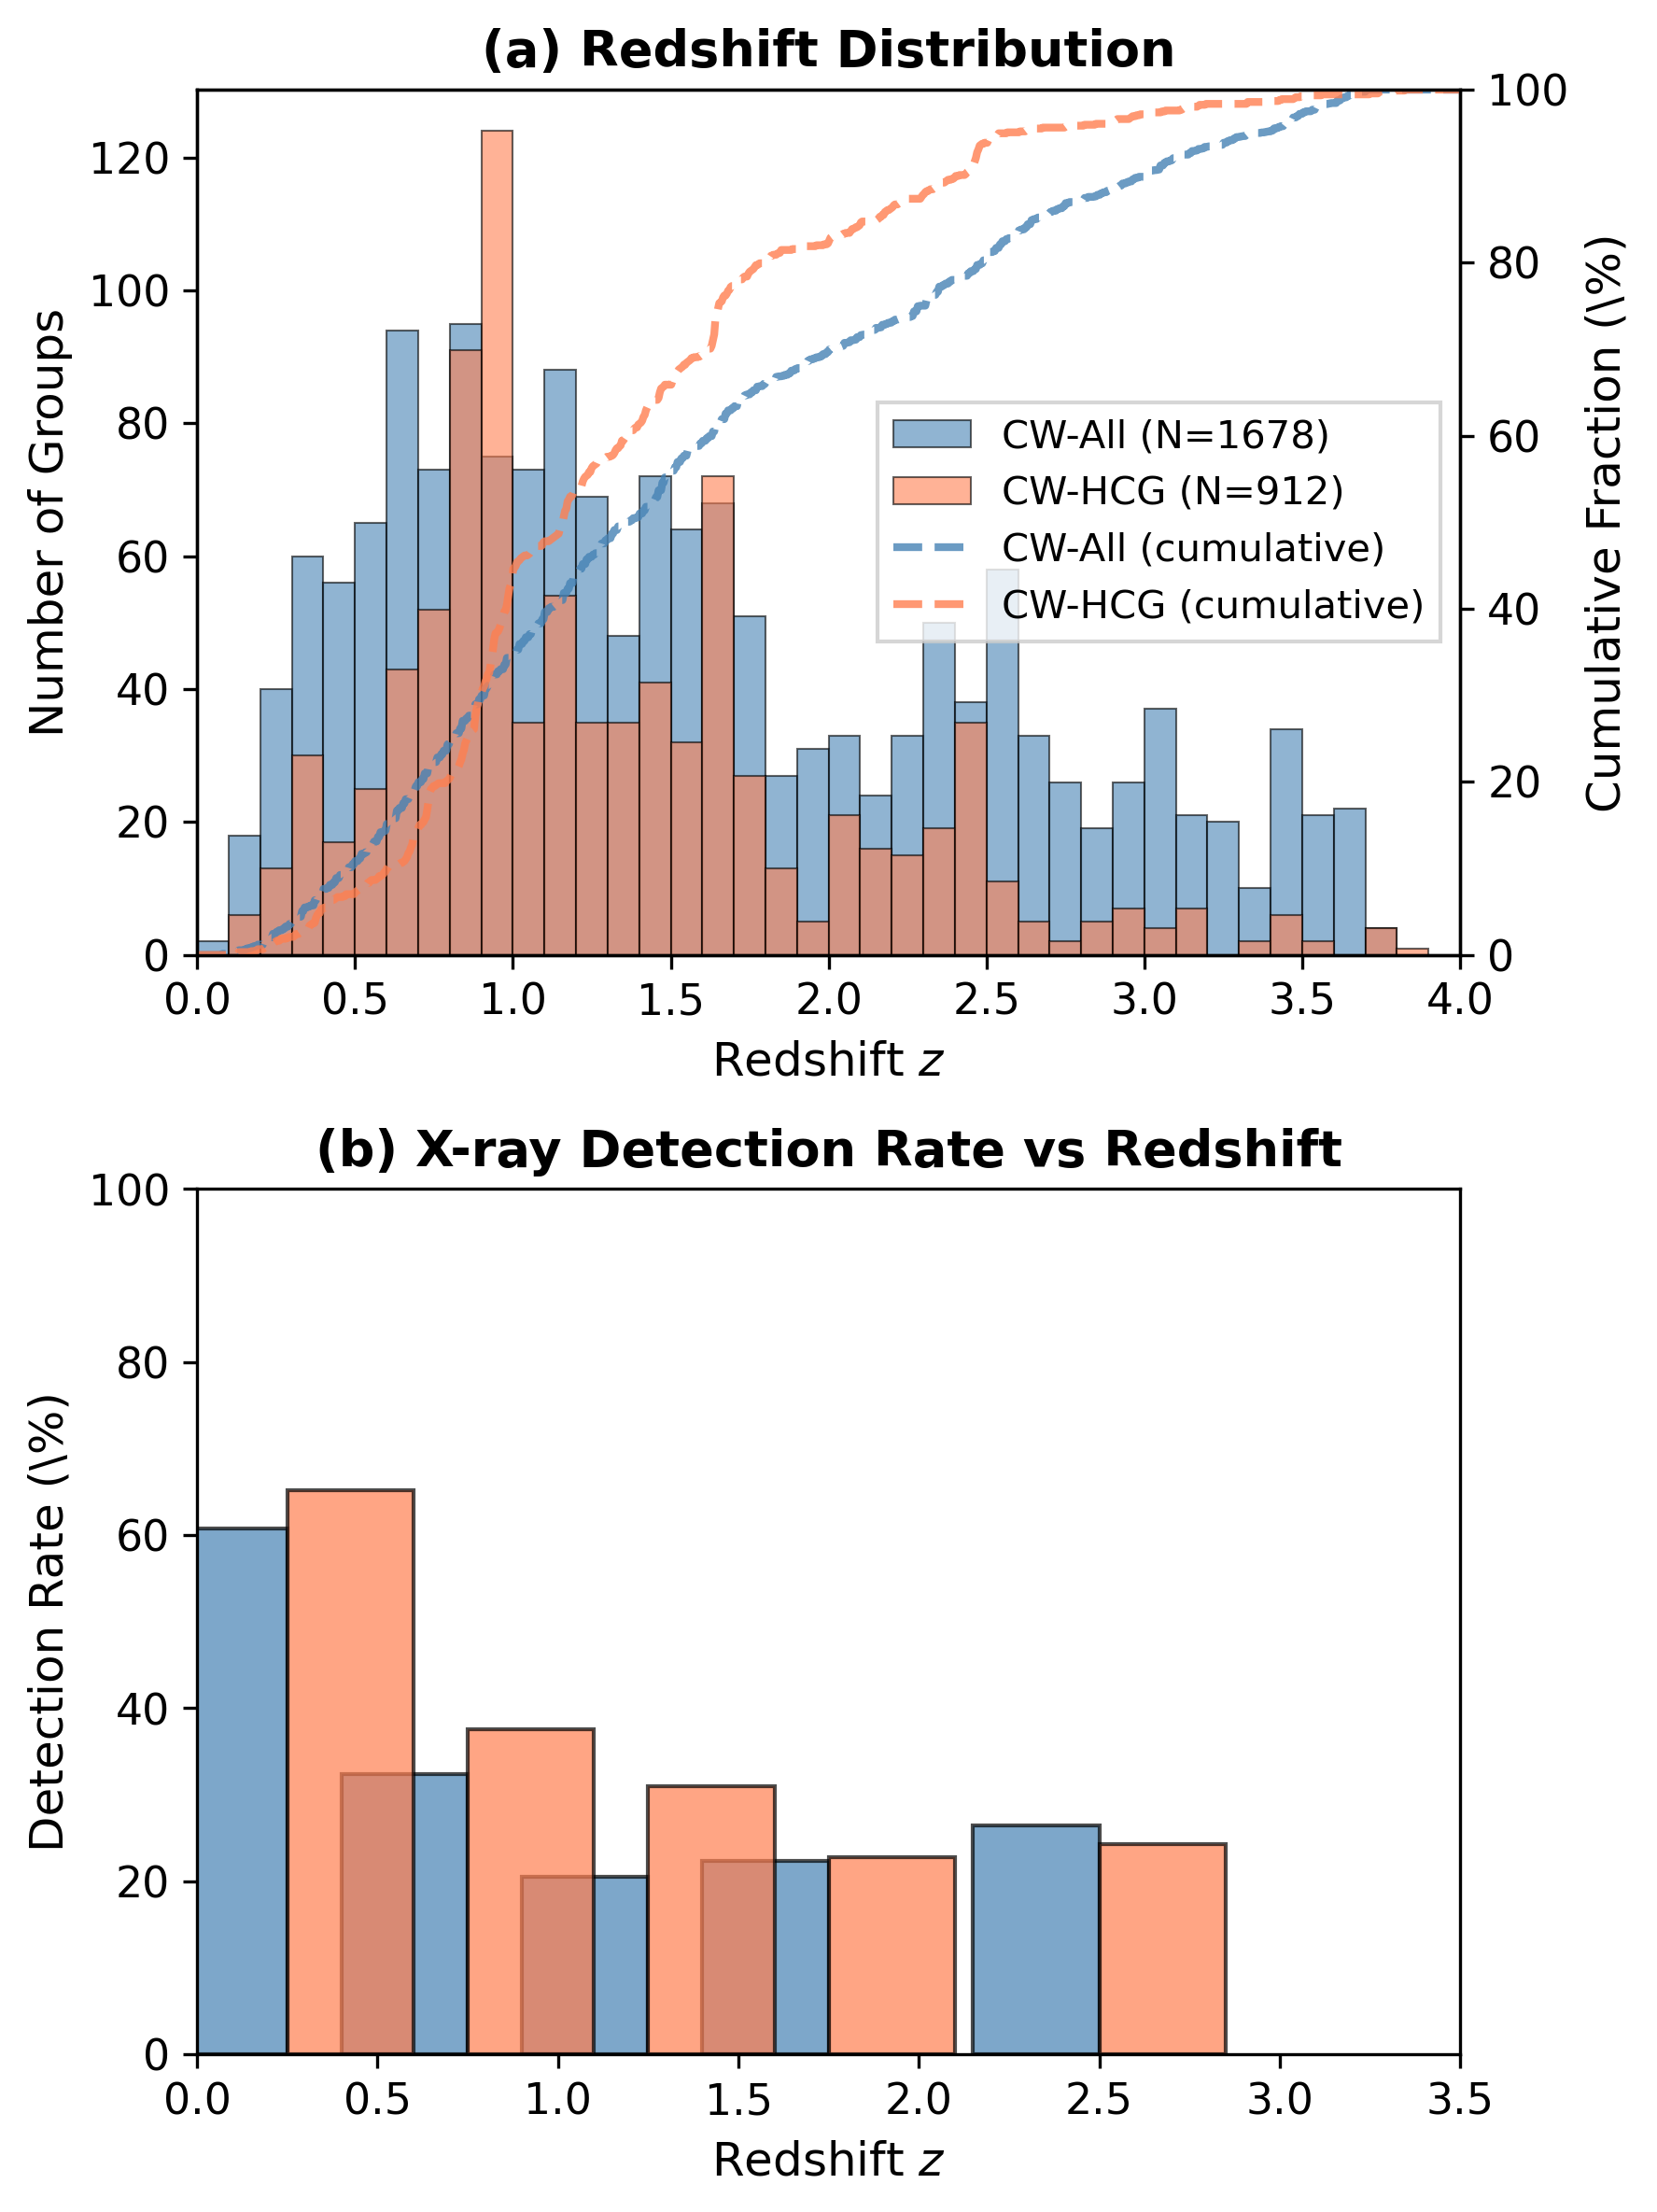
\includegraphics[width=\columnwidth]{figures/redshift_distribution}
\caption{Redshift distribution of the COSMOS-Web group catalogs. Panel~(a) shows the histogram comparison between CW-All (N=1678, blue) and CW-HCG (N=912, orange) samples, with cumulative distributions overlaid as dashed lines on the secondary y-axis (right). Panel~(b) shows the X-ray detection rate as a function of redshift bin for both samples. The distributions reveal that both samples peak at $z \sim 1$--1.5, with CW-HCG showing a slightly lower median redshift ($z \approx 0.97$) compared to CW-All ($z \approx 1.1$).}
\label{fig:redshift_dist}
\end{figure}

\begin{figure*}
\centering
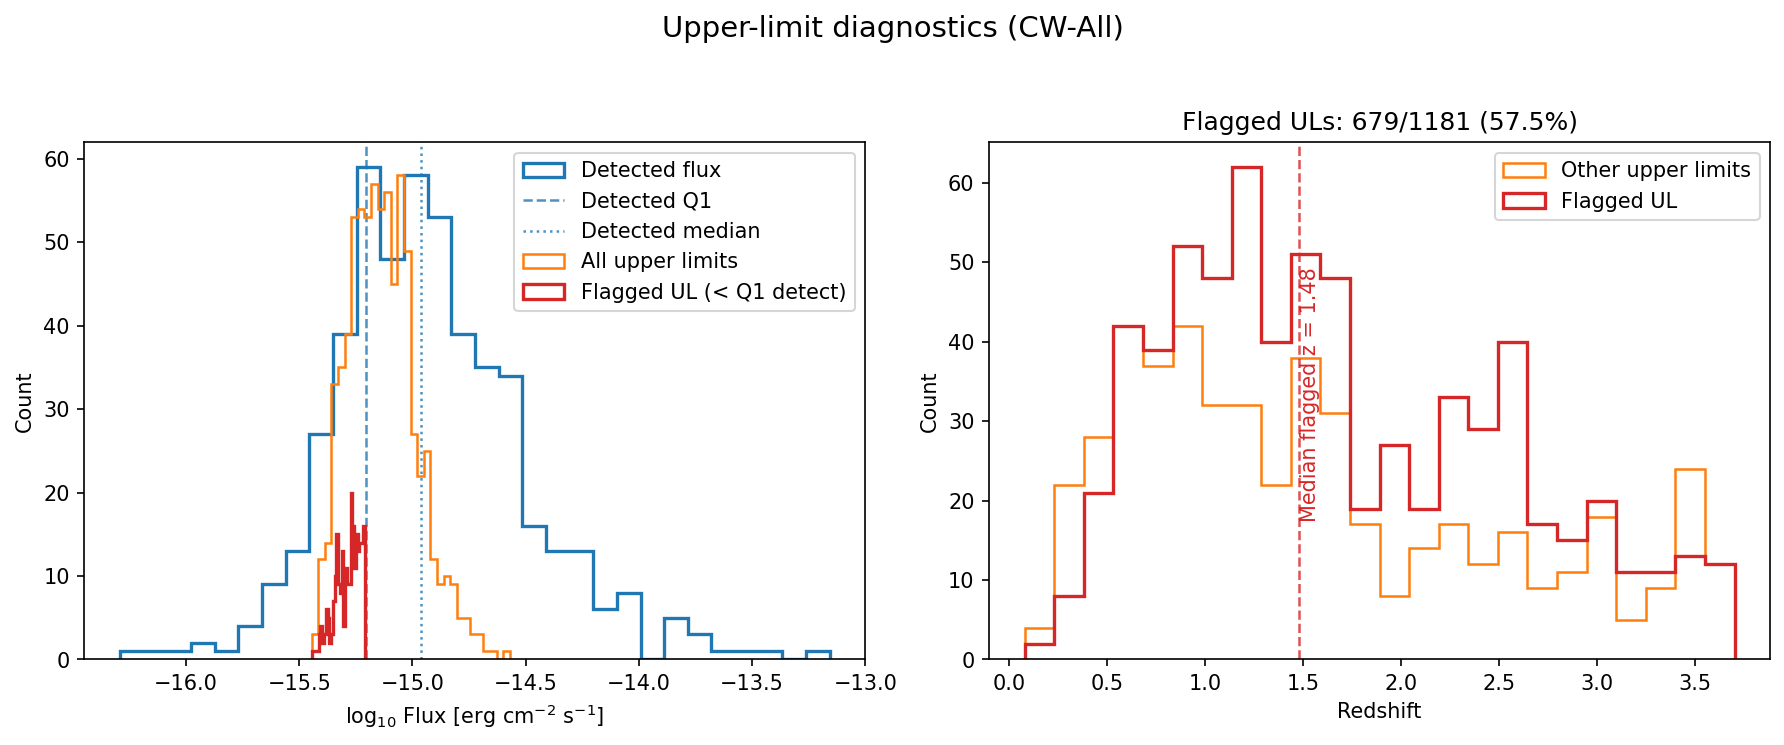
\includegraphics[width=0.49\textwidth]{figures/upper_limit_diagnostics_cw_all}
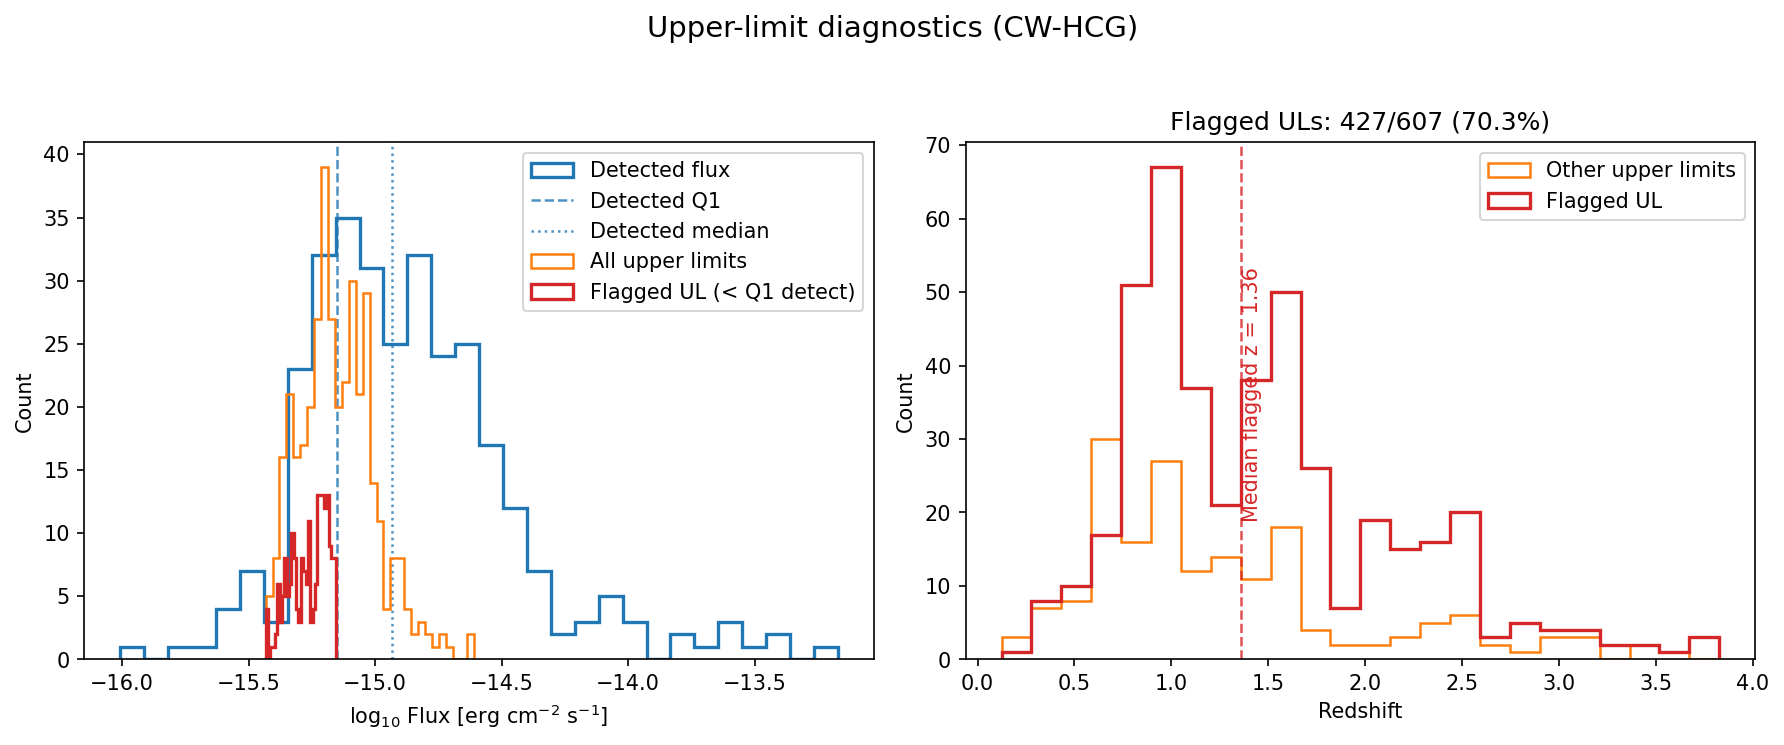
\includegraphics[width=0.49\textwidth]{figures/upper_limit_diagnostics_cw_hcg}
\caption{Upper-limit diagnostics for the CW-All (left) and CW-HCG (right) samples. Left panels: flux distribution histograms showing detected sources (blue), all upper limits (orange), and flagged upper limits (red) that fall below the first quartile of the detected flux distribution. Vertical dashed and dotted lines mark the Q1 and median of detected fluxes. Right panels: redshift distributions of flagged versus unflagged non-detections. Flagged sources are monitored for quality control; masking them changes the stacked fluxes by less than the statistical uncertainties.}
\label{fig:upper_limits}
\end{figure*}

\begin{table}
\caption{Detection summary for COSMOS-Web group samples (SNR $\geq 2.0$). Median properties are computed for the detected subsample.}
\label{tab:detection}
\centering
\begin{tabular}{lrrrcccr}
\hline\hline
Catalog & $N_{\rm tot}$ & $N_{\rm det}$ & Detected (\%) & Median flux (erg cm$^{-2}$ s$^{-1}$) & Median $\log_{10} L_{\rm X}$ & Median $z$ & Median $M_{200}^{L_{\rm X}}$ ($M_{\odot}$) \\
\hline
CW-HCG & 912  & 305 & 33.4 & $1.16 \times 10^{-15}$ & 42.88 & 0.97 & $2.82 \times 10^{13}$ \\
CW-All  & 1678 & 497 & 29.6 & $1.09 \times 10^{-15}$ & 42.97 & 1.10 & $2.88 \times 10^{13}$ \\
\hline
\end{tabular}
\end{table}

\begin{figure*}
\centering
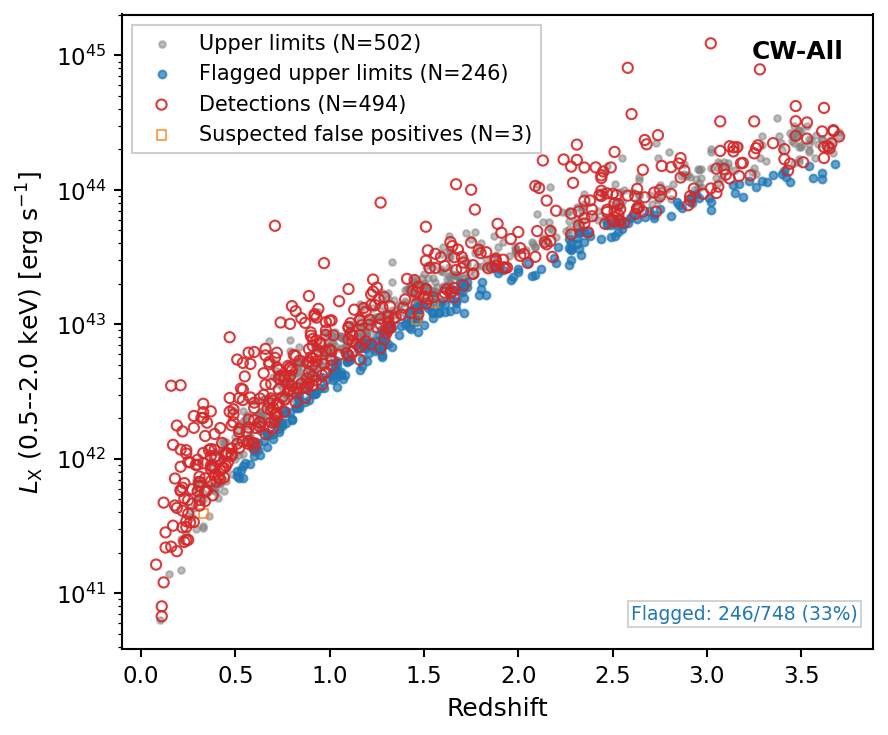
\includegraphics[width=0.49\textwidth]{figures/luminosity_redshift_cw_all}
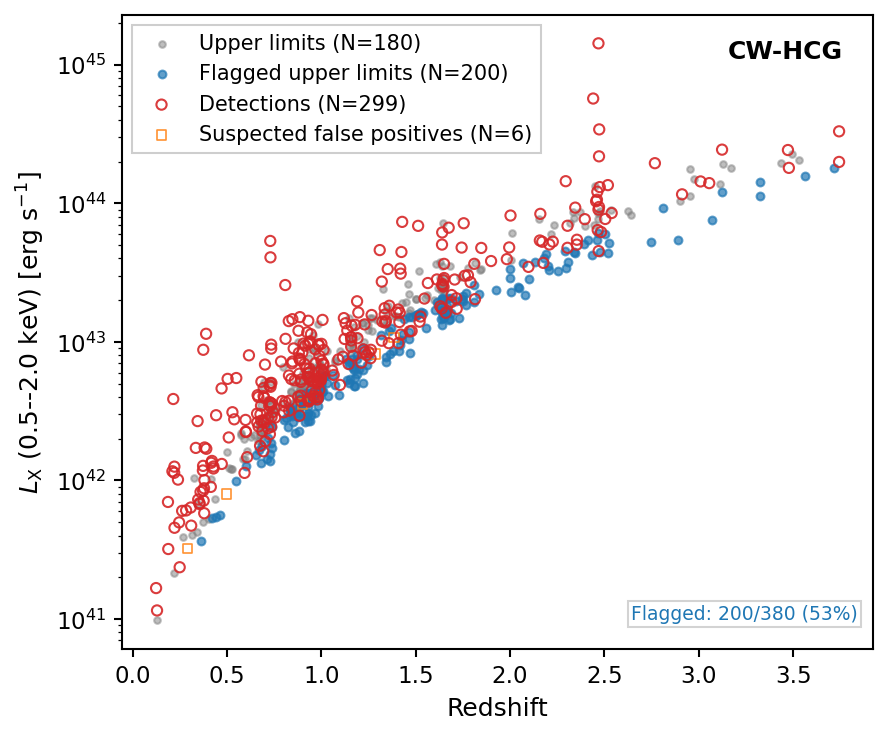
\includegraphics[width=0.49\textwidth]{figures/luminosity_redshift_cw_hcg}
\caption{Rest-frame 0.5--2.0~keV luminosity $L_{\rm X}$ as a function of redshift for the CW-All (left) and CW-HCG (right) samples. Large open circles: individual detections (SNR~$\geq 2.0$). Grey points: non-detections with 95\% Bayesian upper limits; blue points: upper limits below the first quartile of the detected flux distribution (flagged). Orange squares: stacked median $L_{\rm X}$ per redshift bin (Tables~\ref{tab:stacking_all} and~\ref{tab:stacking_hcg}). This figure is the primary diagnostic for X-ray luminosity across the sample (see \S\ref{sec:LX_z}).}
\label{fig:LX_z}
\end{figure*}

\begin{table*}
\caption{Stacked X-ray measurements for the COSMOS-Web ``All'' sample. Fluxes are mean per-source values and uncertainties reflect bootstrap errors.}
\label{tab:stacking_all}
\centering
\begin{tabular}{cccrrcrrr}
\hline\hline
$z_{\rm min}$ & $z_{\rm max}$ & $\langle z \rangle$ & $N_{\rm src}$ & SNR & \multicolumn{2}{c}{Flux (erg cm$^{-2}$ s$^{-1}$)} & \multicolumn{2}{c}{$L_{\rm X}$ (erg s$^{-1}$)} \\
 &  &  &  &  & Flux & $\sigma_F$ & $L_{\rm X}$ & $\sigma_L$ \\
\hline
0.25 & 0.50 & 0.38 & 135 & 12.93 & $1.81\times10^{-15}$ & $1.40\times10^{-16}$ & $1.14\times10^{42}$ & $8.81\times10^{40}$ \\
0.50 & 0.75 & 0.63 & 193 & 14.75 & $7.92\times10^{-16}$ & $5.37\times10^{-17}$ & $1.81\times10^{42}$ & $1.23\times10^{41}$ \\
0.75 & 1.00 & 0.88 & 223 & 12.55 & $5.89\times10^{-16}$ & $4.69\times10^{-17}$ & $3.27\times10^{42}$ & $2.60\times10^{41}$ \\
1.00 & 1.25 & 1.12 & 194 & 16.85 & $5.50\times10^{-16}$ & $3.26\times10^{-17}$ & $5.93\times10^{42}$ & $3.52\times10^{41}$ \\
1.25 & 1.50 & 1.40 & 156 & 11.89 & $4.74\times10^{-16}$ & $3.99\times10^{-17}$ & $9.32\times10^{42}$ & $7.83\times10^{41}$ \\
1.50 & 1.75 & 1.63 &  96 & 16.31 & $5.58\times10^{-16}$ & $3.42\times10^{-17}$ & $1.67\times10^{43}$ & $1.02\times10^{42}$ \\
1.75 & 2.00 & 1.88 &  49 &  5.69 & $3.06\times10^{-16}$ & $5.37\times10^{-17}$ & $1.36\times10^{43}$ & $2.38\times10^{42}$ \\
2.00 & 2.50 & 2.25 & 109 &  9.38 & $5.01\times10^{-16}$ & $5.34\times10^{-17}$ & $3.79\times10^{43}$ & $4.04\times10^{42}$ \\
2.50 & 3.80 & 3.15 & 211 & 27.70 & $6.20\times10^{-16}$ & $2.24\times10^{-17}$ & $1.02\times10^{44}$ & $3.69\times10^{42}$ \\
\hline
\end{tabular}
\tablefoot{Columns also include $\log_{10} M_{200}$ (dex): see full electronic table.}
\end{table*}

\begin{table*}
\caption{Stacked X-ray measurements for the CW-HCG sample.}
\label{tab:stacking_hcg}
\centering
\begin{tabular}{cccrrcrrr}
\hline\hline
$z_{\rm min}$ & $z_{\rm max}$ & $\langle z \rangle$ & $N_{\rm src}$ & SNR & \multicolumn{2}{c}{Flux (erg cm$^{-2}$ s$^{-1}$)} & \multicolumn{2}{c}{$L_{\rm X}$ (erg s$^{-1}$)} \\
 &  &  &  &  & Flux & $\sigma_F$ & $L_{\rm X}$ & $\sigma_L$ \\
\hline
0.25 & 0.50 & 0.38 &  51 &  6.53 & $2.62\times10^{-15}$ & $4.02\times10^{-16}$ & $1.64\times10^{42}$ & $2.51\times10^{41}$ \\
0.50 & 0.75 & 0.63 & 112 & 11.90 & $1.07\times10^{-15}$ & $8.95\times10^{-17}$ & $3.02\times10^{42}$ & $2.54\times10^{41}$ \\
0.75 & 1.00 & 0.88 & 223 & 14.07 & $6.23\times10^{-16}$ & $4.43\times10^{-17}$ & $3.82\times10^{42}$ & $2.72\times10^{41}$ \\
1.00 & 1.25 & 1.16 & 112 & 10.30 & $4.34\times10^{-16}$ & $4.21\times10^{-17}$ & $5.06\times10^{42}$ & $4.92\times10^{41}$ \\
1.25 & 1.50 & 1.39 &  88 &  6.01 & $4.94\times10^{-16}$ & $8.22\times10^{-17}$ & $9.61\times10^{42}$ & $1.60\times10^{42}$ \\
1.50 & 1.75 & 1.64 &  82 &  9.06 & $4.34\times10^{-16}$ & $4.79\times10^{-17}$ & $1.32\times10^{43}$ & $1.45\times10^{42}$ \\
1.75 & 2.00 & 1.88 &  23 &  3.66 & $4.51\times10^{-16}$ & $1.23\times10^{-16}$ & $1.80\times10^{43}$ & $4.93\times10^{42}$ \\
2.00 & 2.50 & 2.25 &  80 &  6.07 & $2.16\times10^{-16}$ & $3.56\times10^{-17}$ & $2.09\times10^{43}$ & $3.43\times10^{42}$ \\
2.50 & 3.80 & 3.15 &  39 &  6.44 & $3.98\times10^{-16}$ & $6.18\times10^{-17}$ & $6.18\times10^{43}$ & $9.61\times10^{42}$ \\
\hline
\end{tabular}
\end{table*}

\begin{figure}
\centering
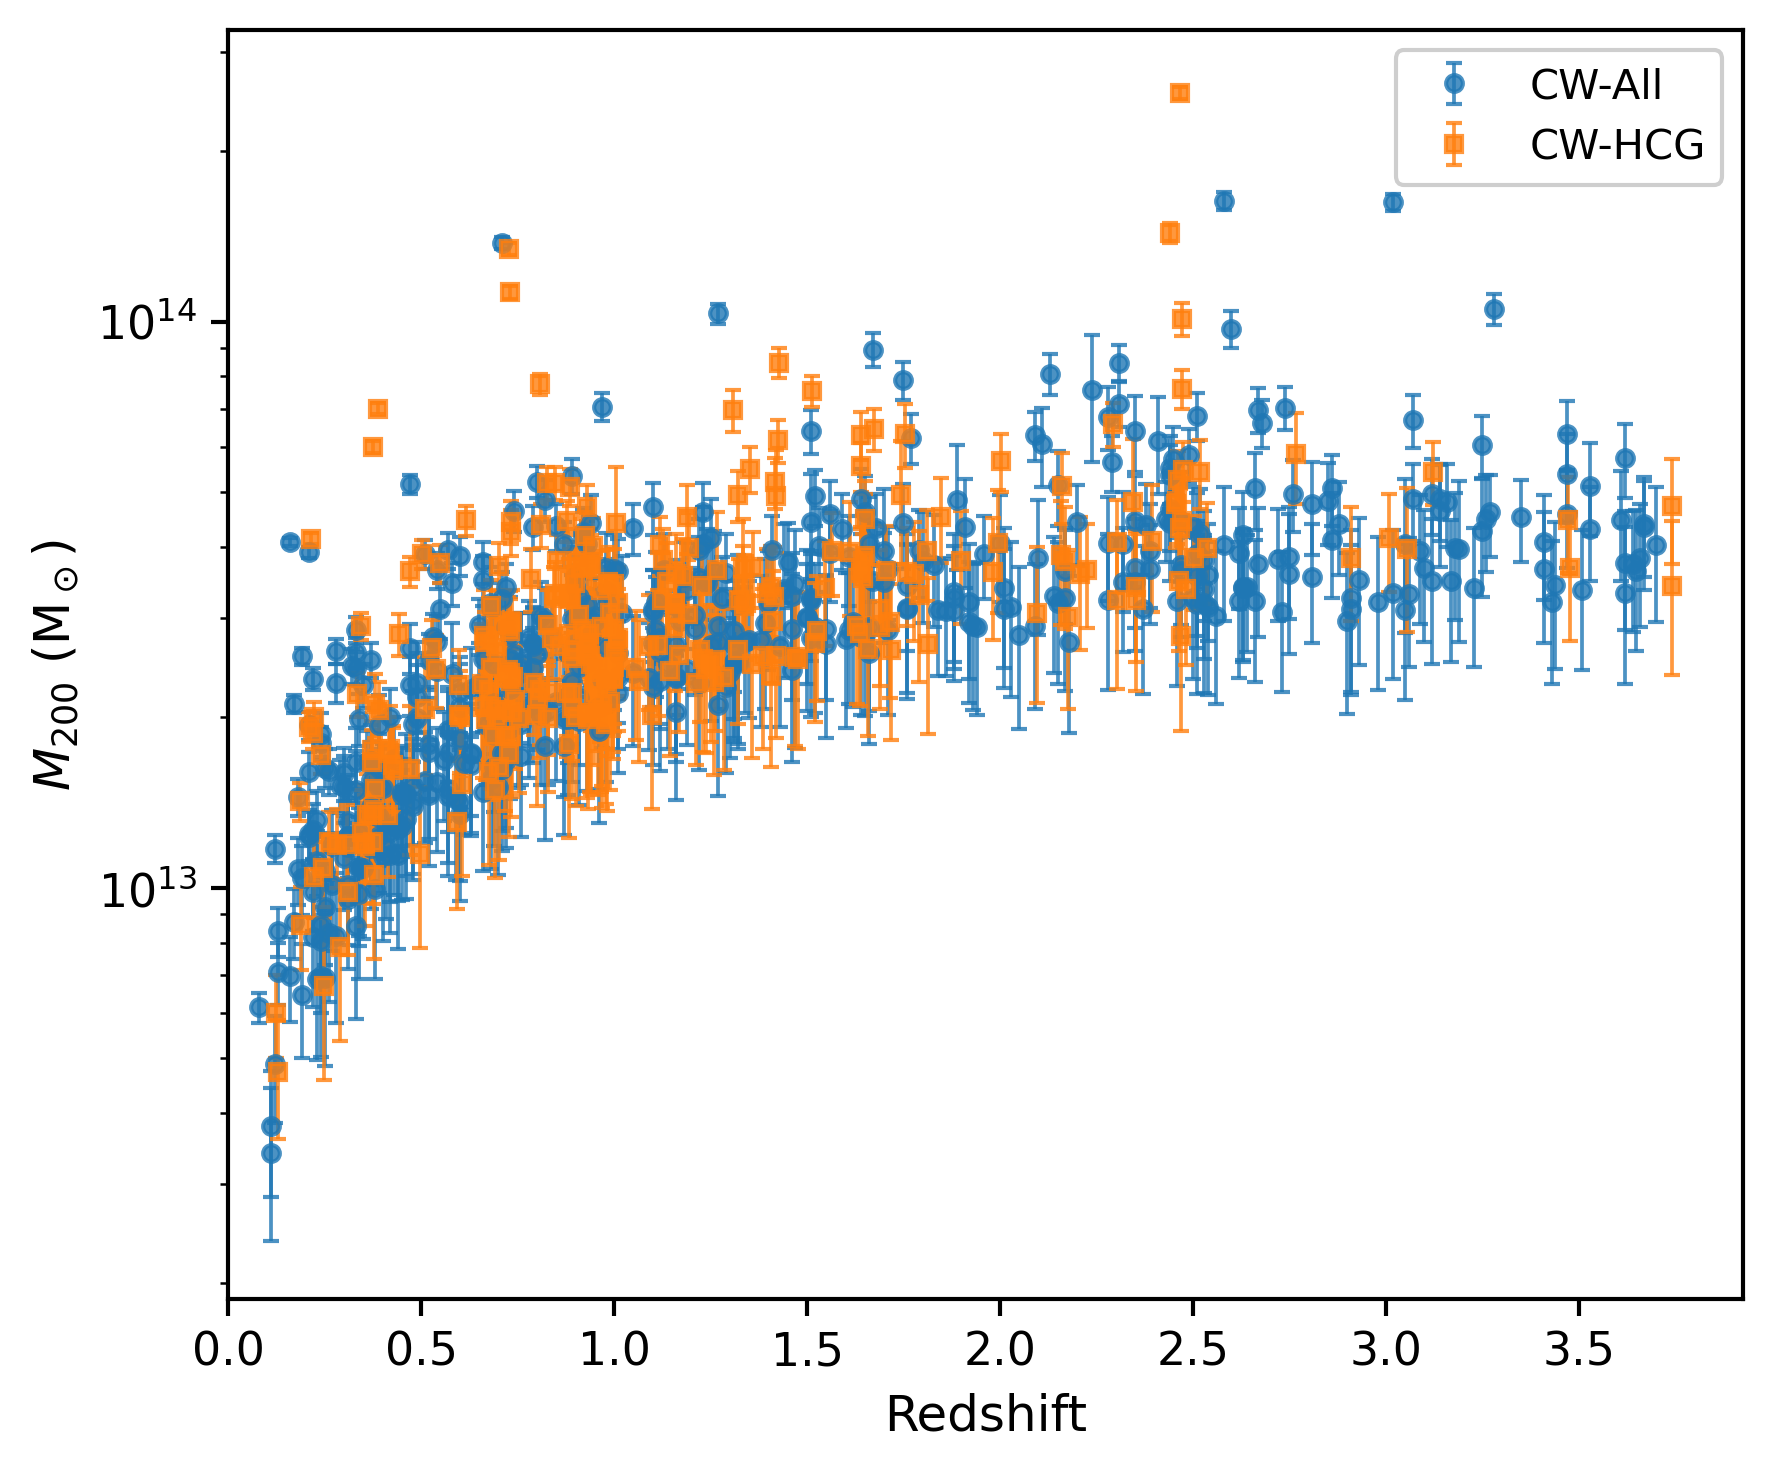
\includegraphics[width=\columnwidth]{figures/m200_redshift_detections}
\caption{Halo mass $M_{200}^{L_{\rm X}}$ as a function of redshift for detected groups in the CW-All (blue circles) and CW-HCG (orange squares) samples, using the weak-lensing calibrated $M$--$L_{\rm X}$ scaling relation of \citet{Leauthaud2010}. The points illustrate the mass range and redshift leverage of our X-ray-detected systems.}
\label{fig:M200_z}
\end{figure}

\begin{figure*}
\centering
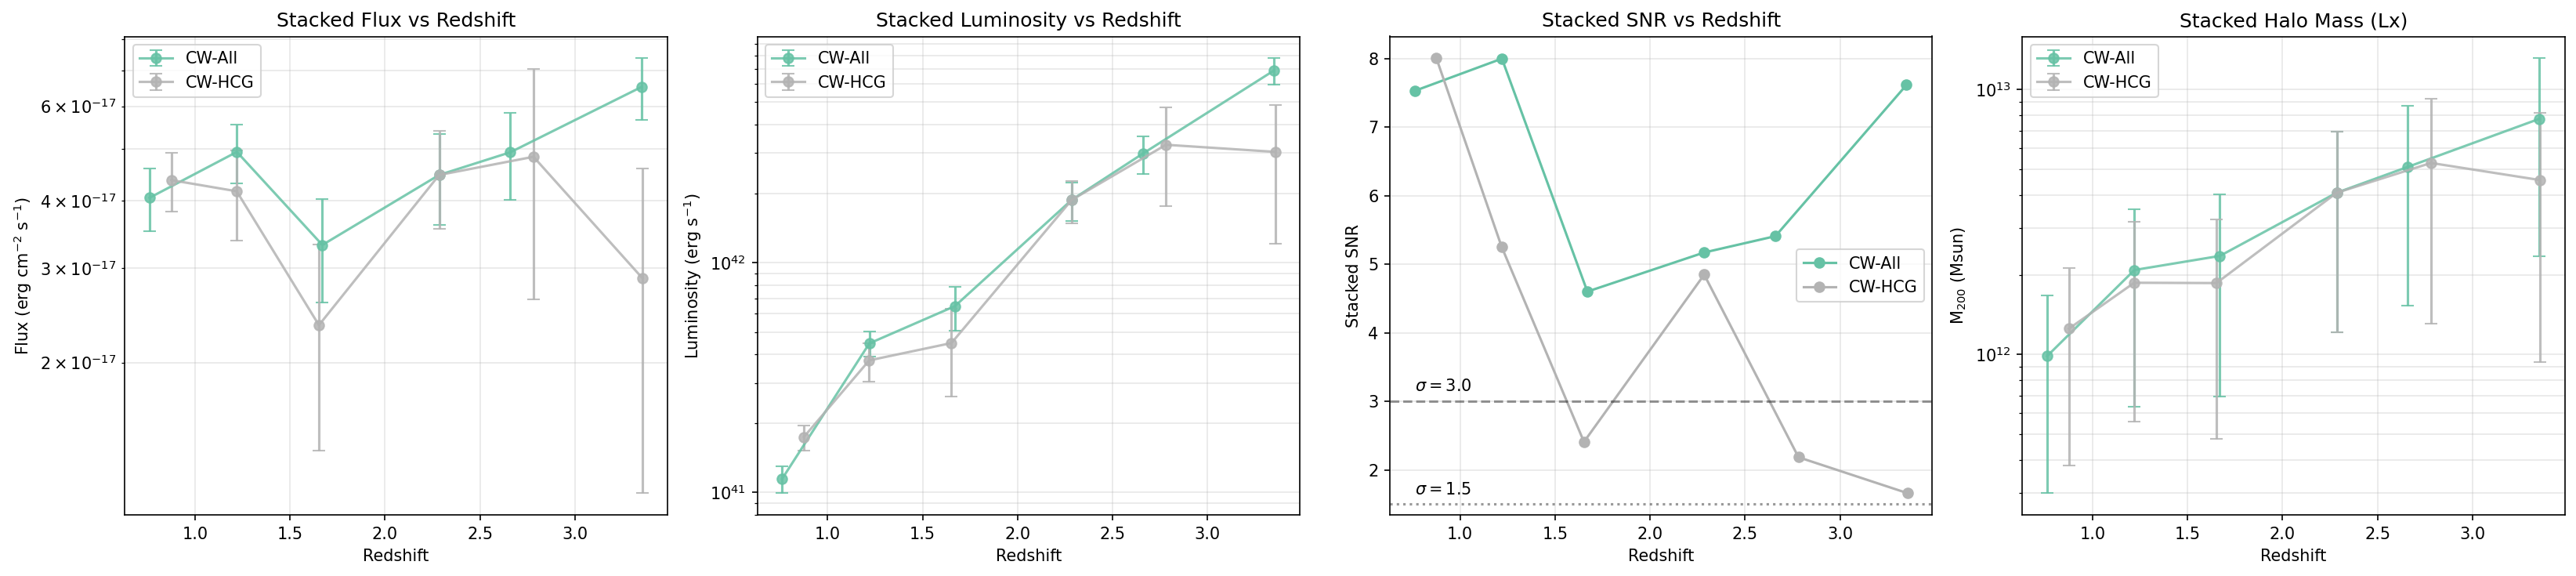
\includegraphics[width=\textwidth]{figures/stacking_comparison_multi}
\caption{Comparison of stacked X-ray properties as a function of redshift for stacks built from all groups in each bin (solid lines) versus stacks restricted to individually detected systems (dashed lines), for the CW-All (blue circles) and CW-HCG (orange squares) samples. From left to right the panels show rest-frame $L_{\rm X}$, observed-frame flux, stacked SNR, and halo mass $M_{200}^{L_{\rm X}}$. The close agreement between the all-groups and detections-only curves at $z \lesssim 2$ indicates that the stacked signals are representative of the full group population rather than being driven solely by a small number of bright detections.}
\label{fig:stacking}
\end{figure*}

% Appendix figures

\begin{figure*}
\centering
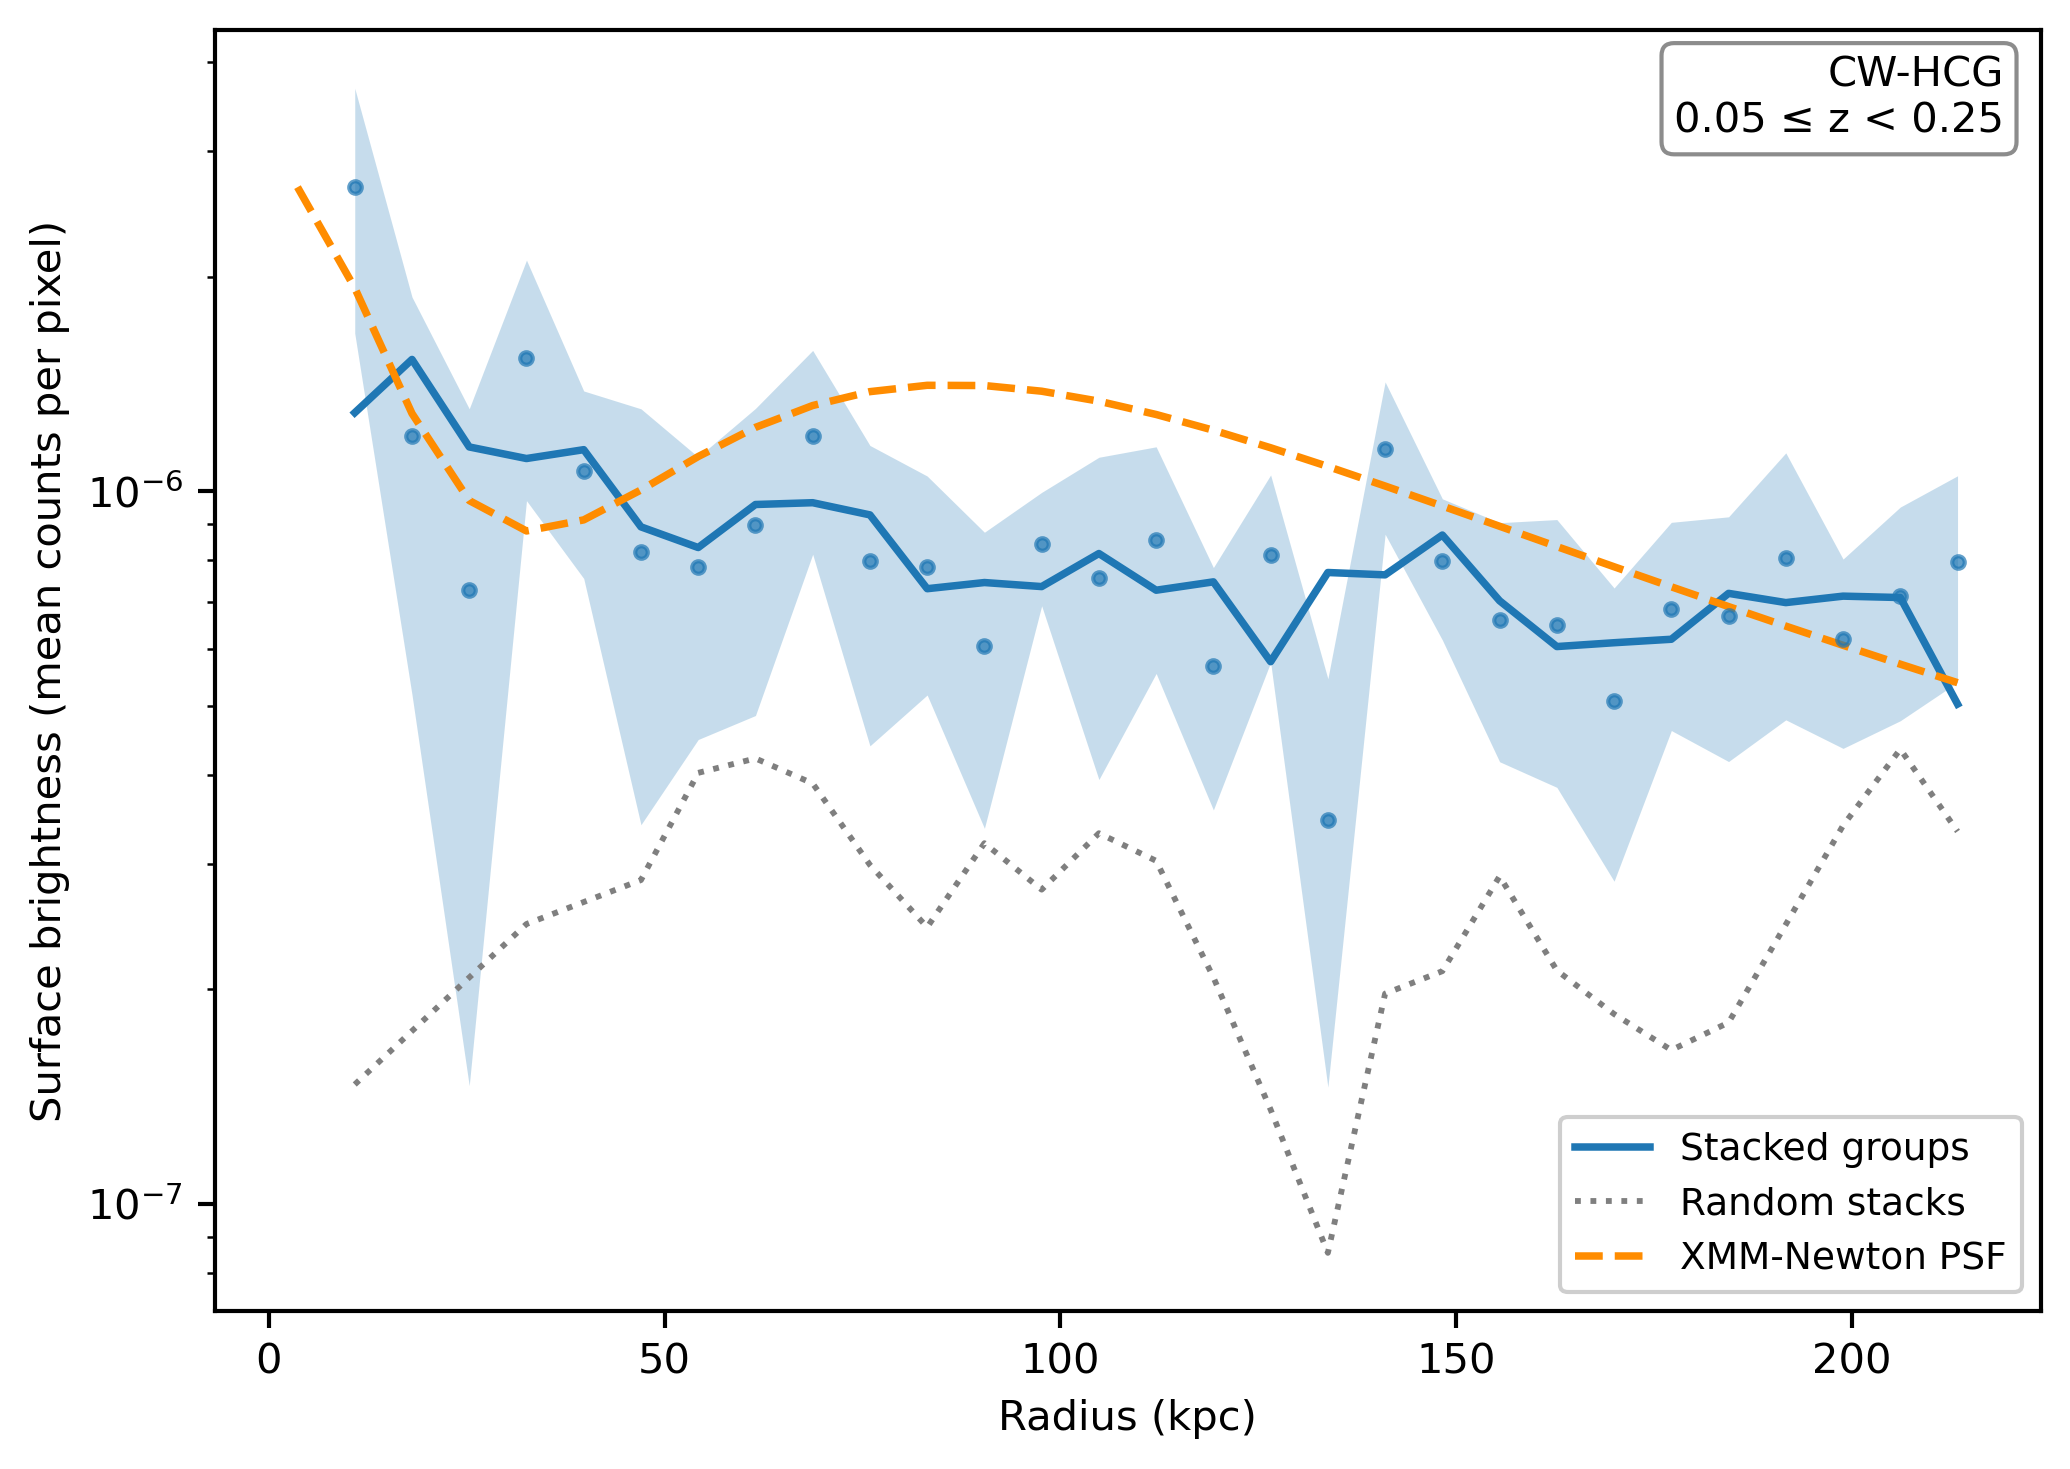
\includegraphics[width=0.32\textwidth]{figures/stacking_radial_profiles_z_0.05_0.25}
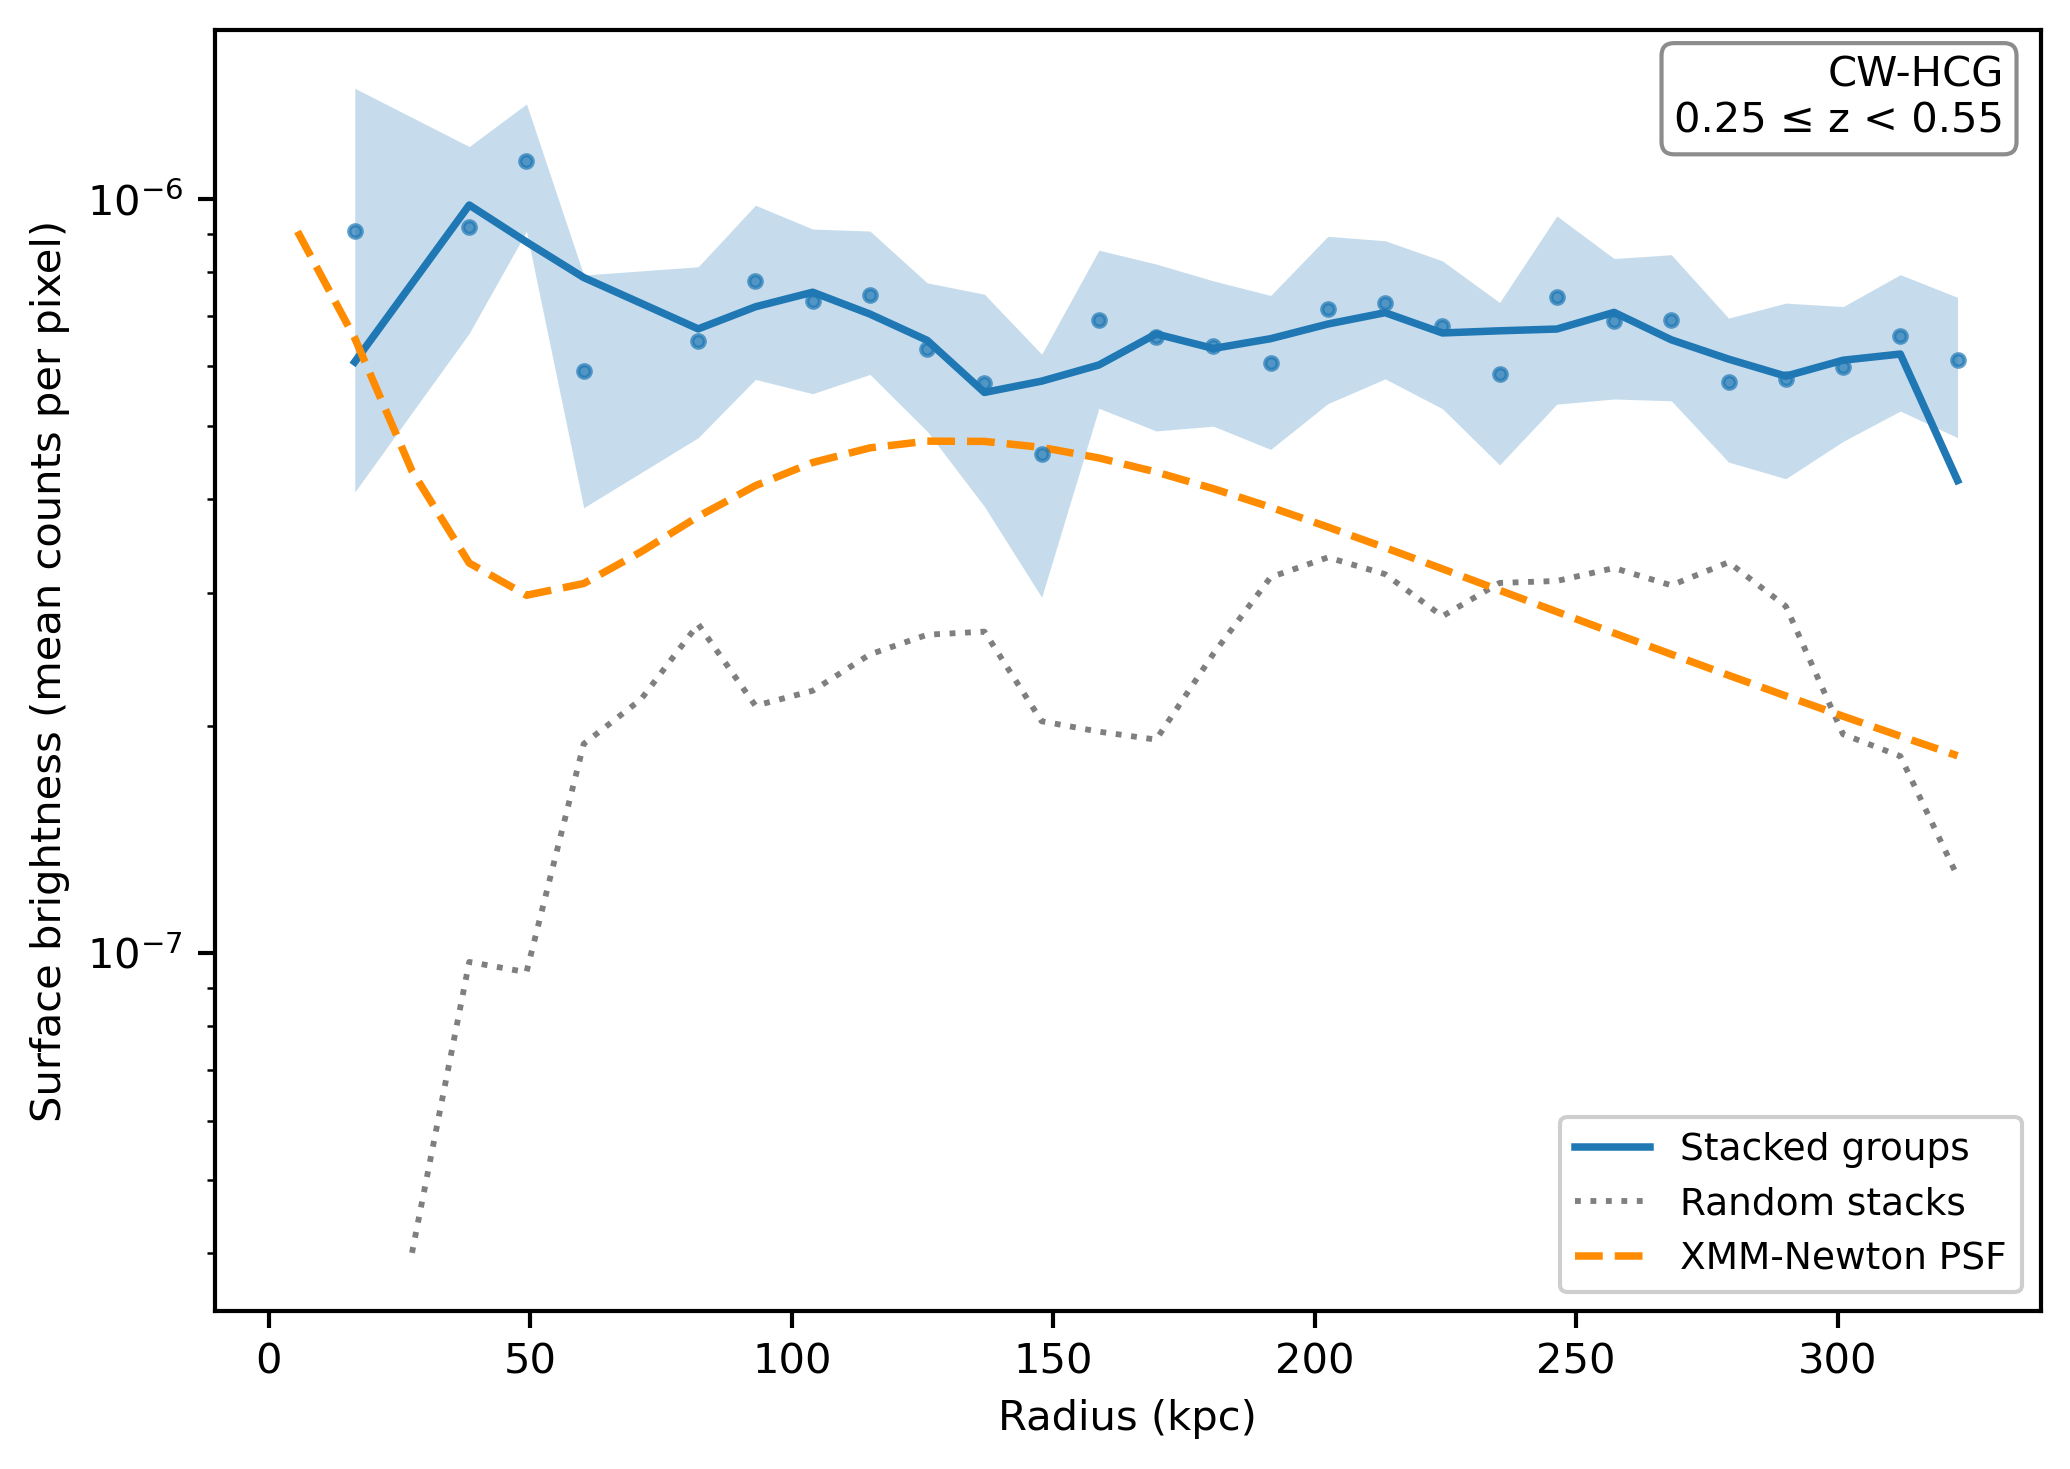
\includegraphics[width=0.32\textwidth]{figures/stacking_radial_profiles_z_0.25_0.55}
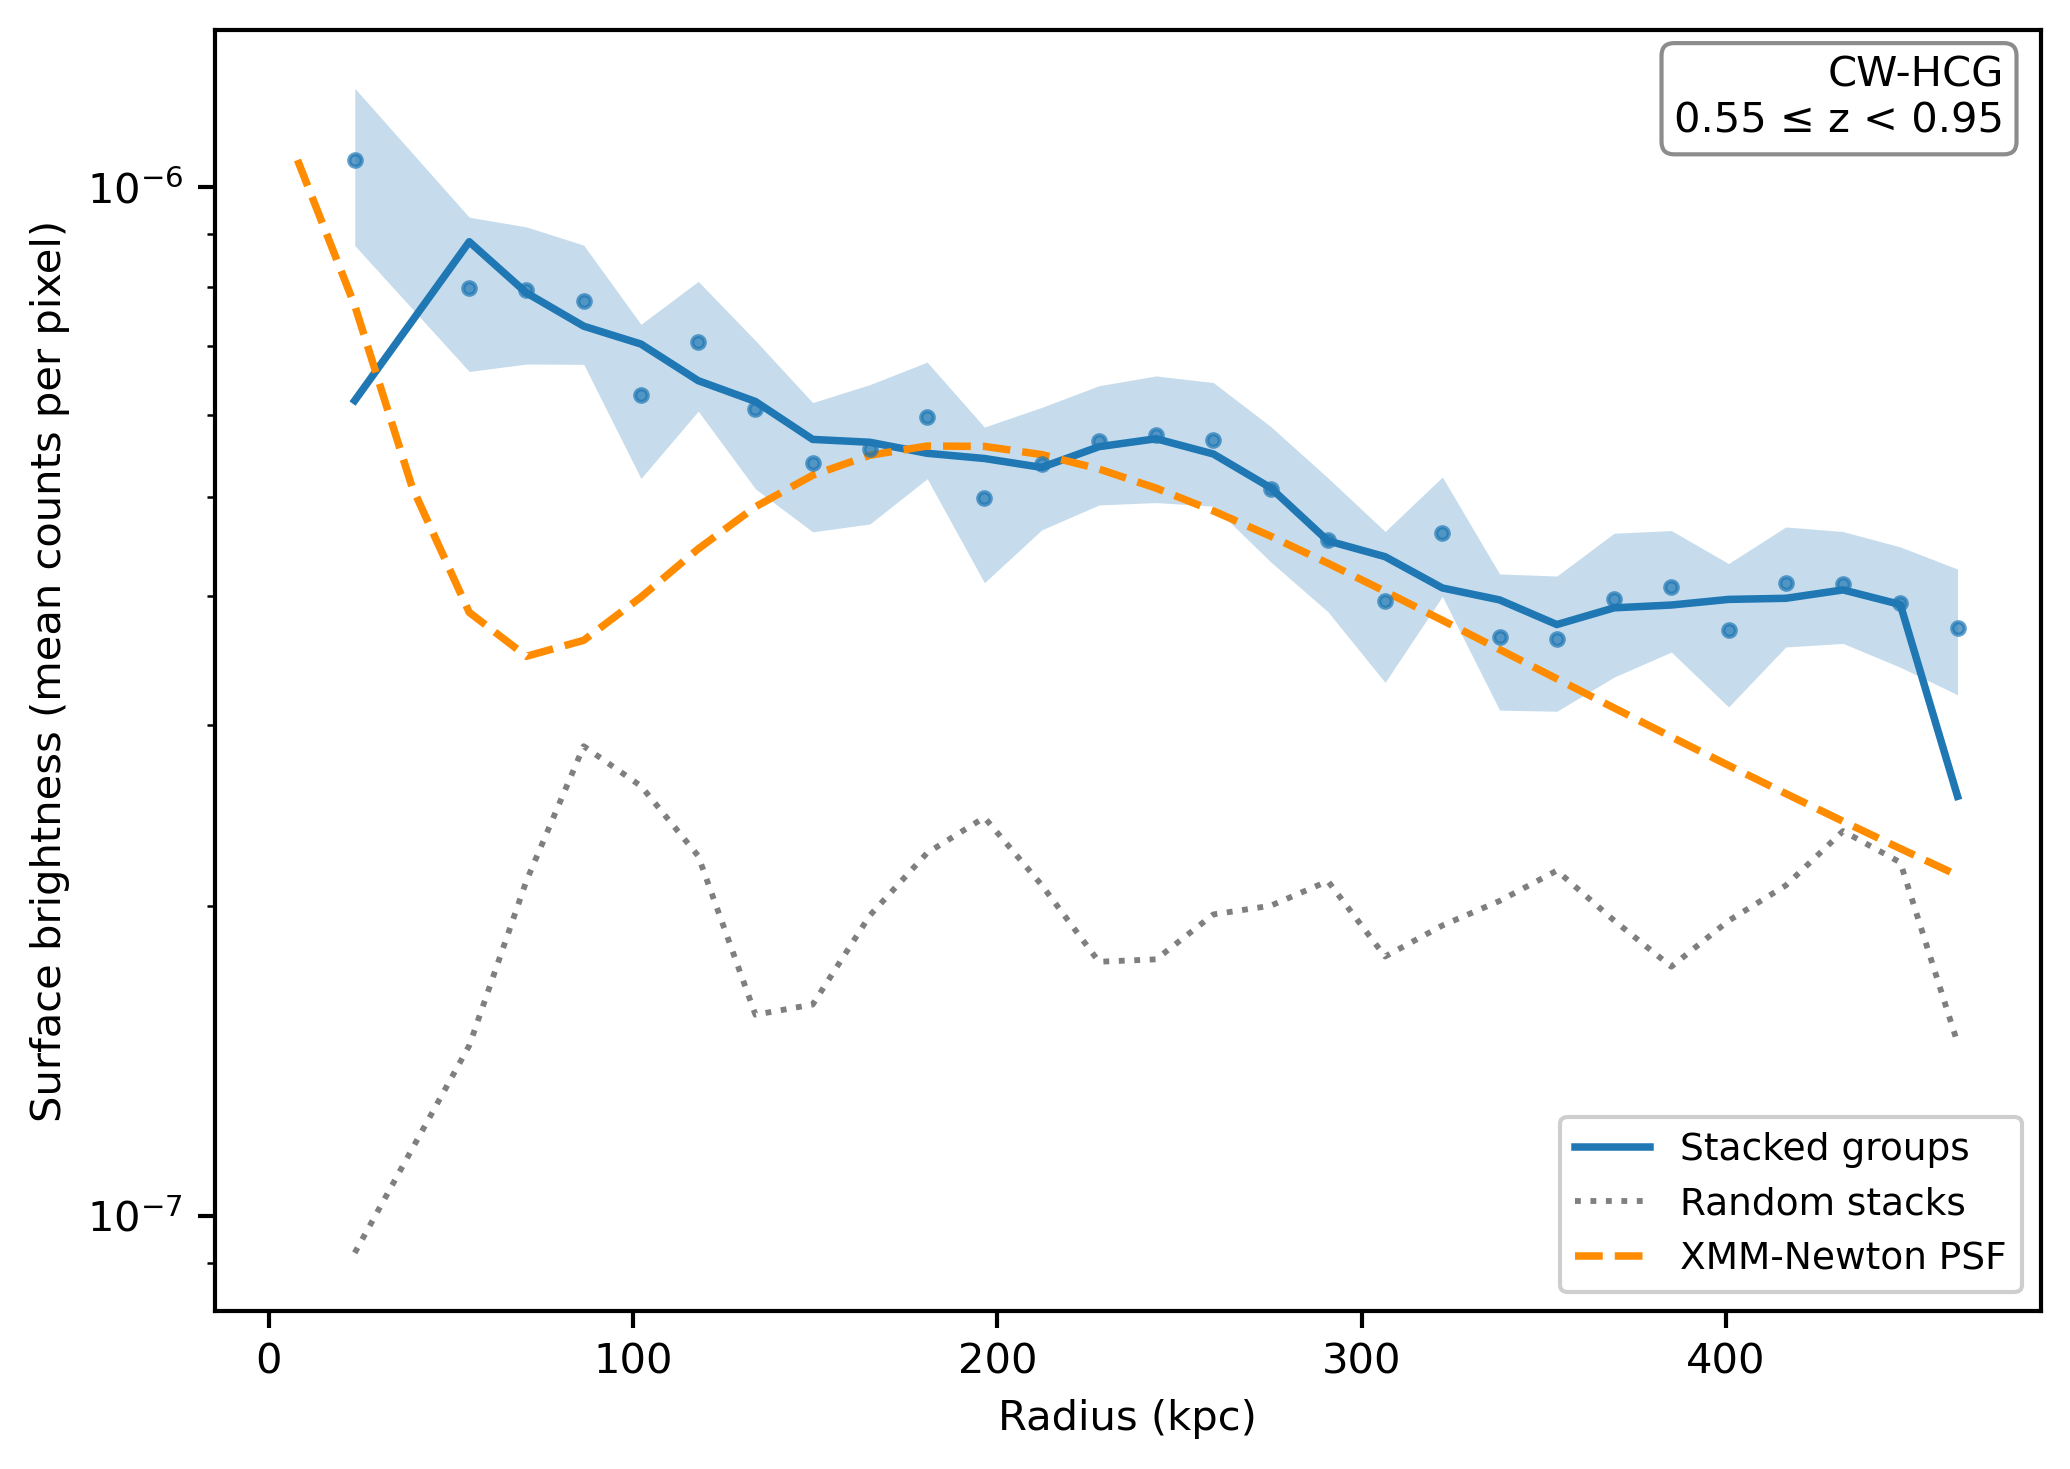
\includegraphics[width=0.32\textwidth]{figures/stacking_radial_profiles_z_0.55_0.95}
\caption{Representative stacked 0.5--2~keV radial surface-brightness profiles for the full COSMOS-Web group sample (CW-All) in three redshift bins, as indicated in each panel. Blue points and lines show the stacked group profiles with $1\sigma$ uncertainties, the grey dotted curves show random-stack null tests, and the orange dashed lines show the analytic XMM--Newton PSF model at the median redshift of each bin, normalised to the central surface brightness.}
\label{fig:profiles_all}
\end{figure*}

\begin{figure*}
\centering
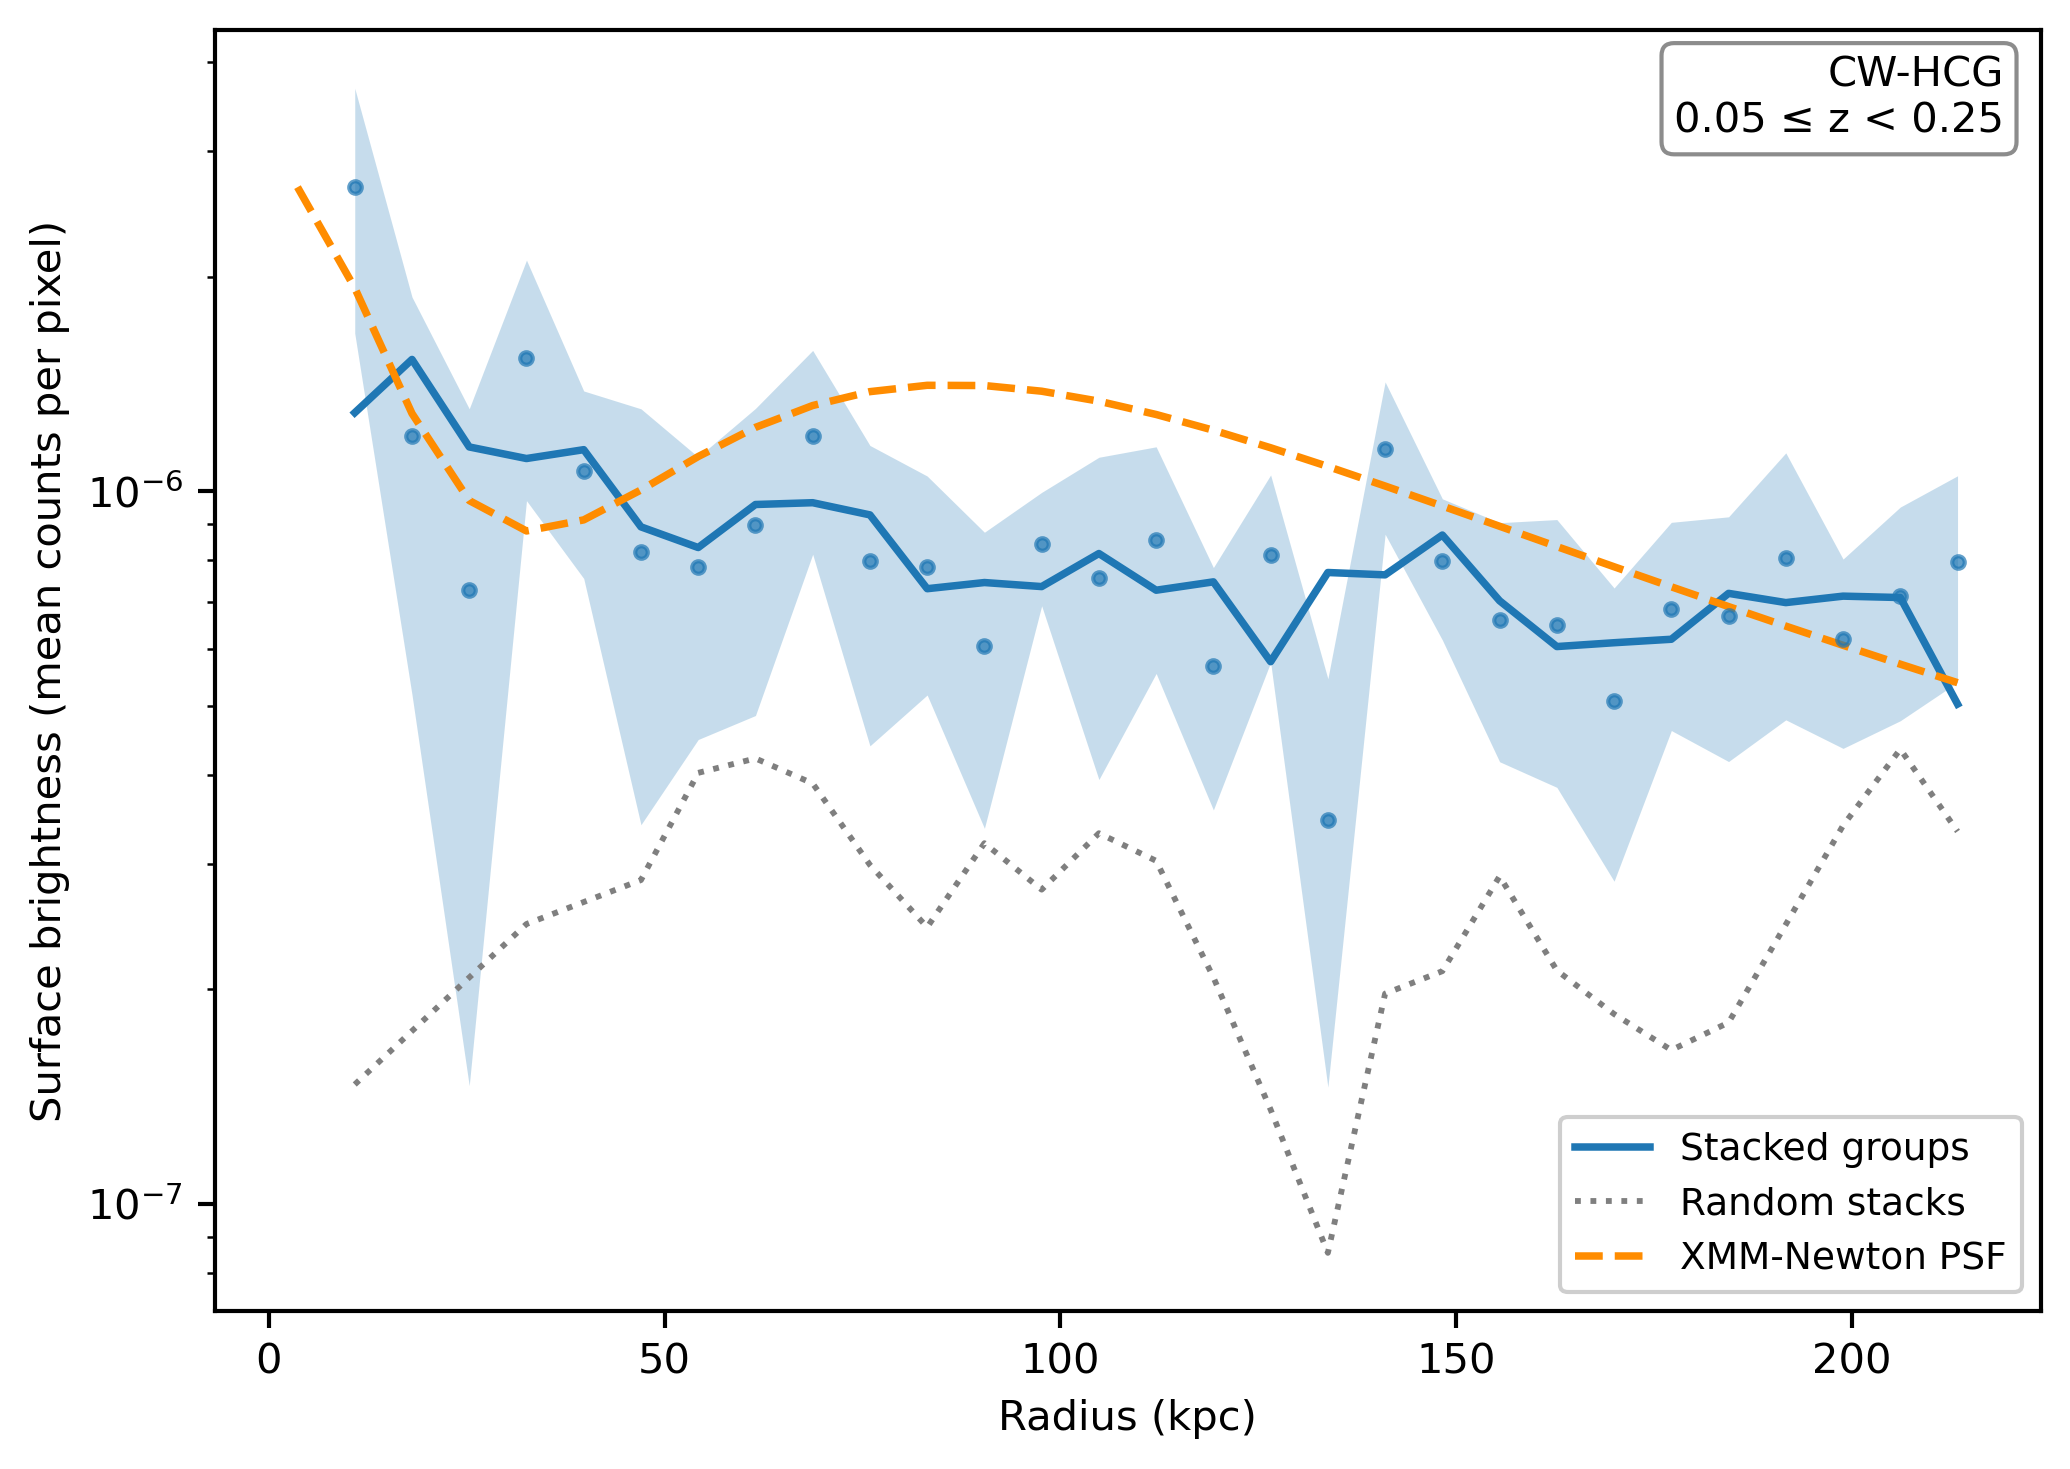
\includegraphics[width=0.32\textwidth]{figures/stacking_radial_profiles_z_0.05_0.25}
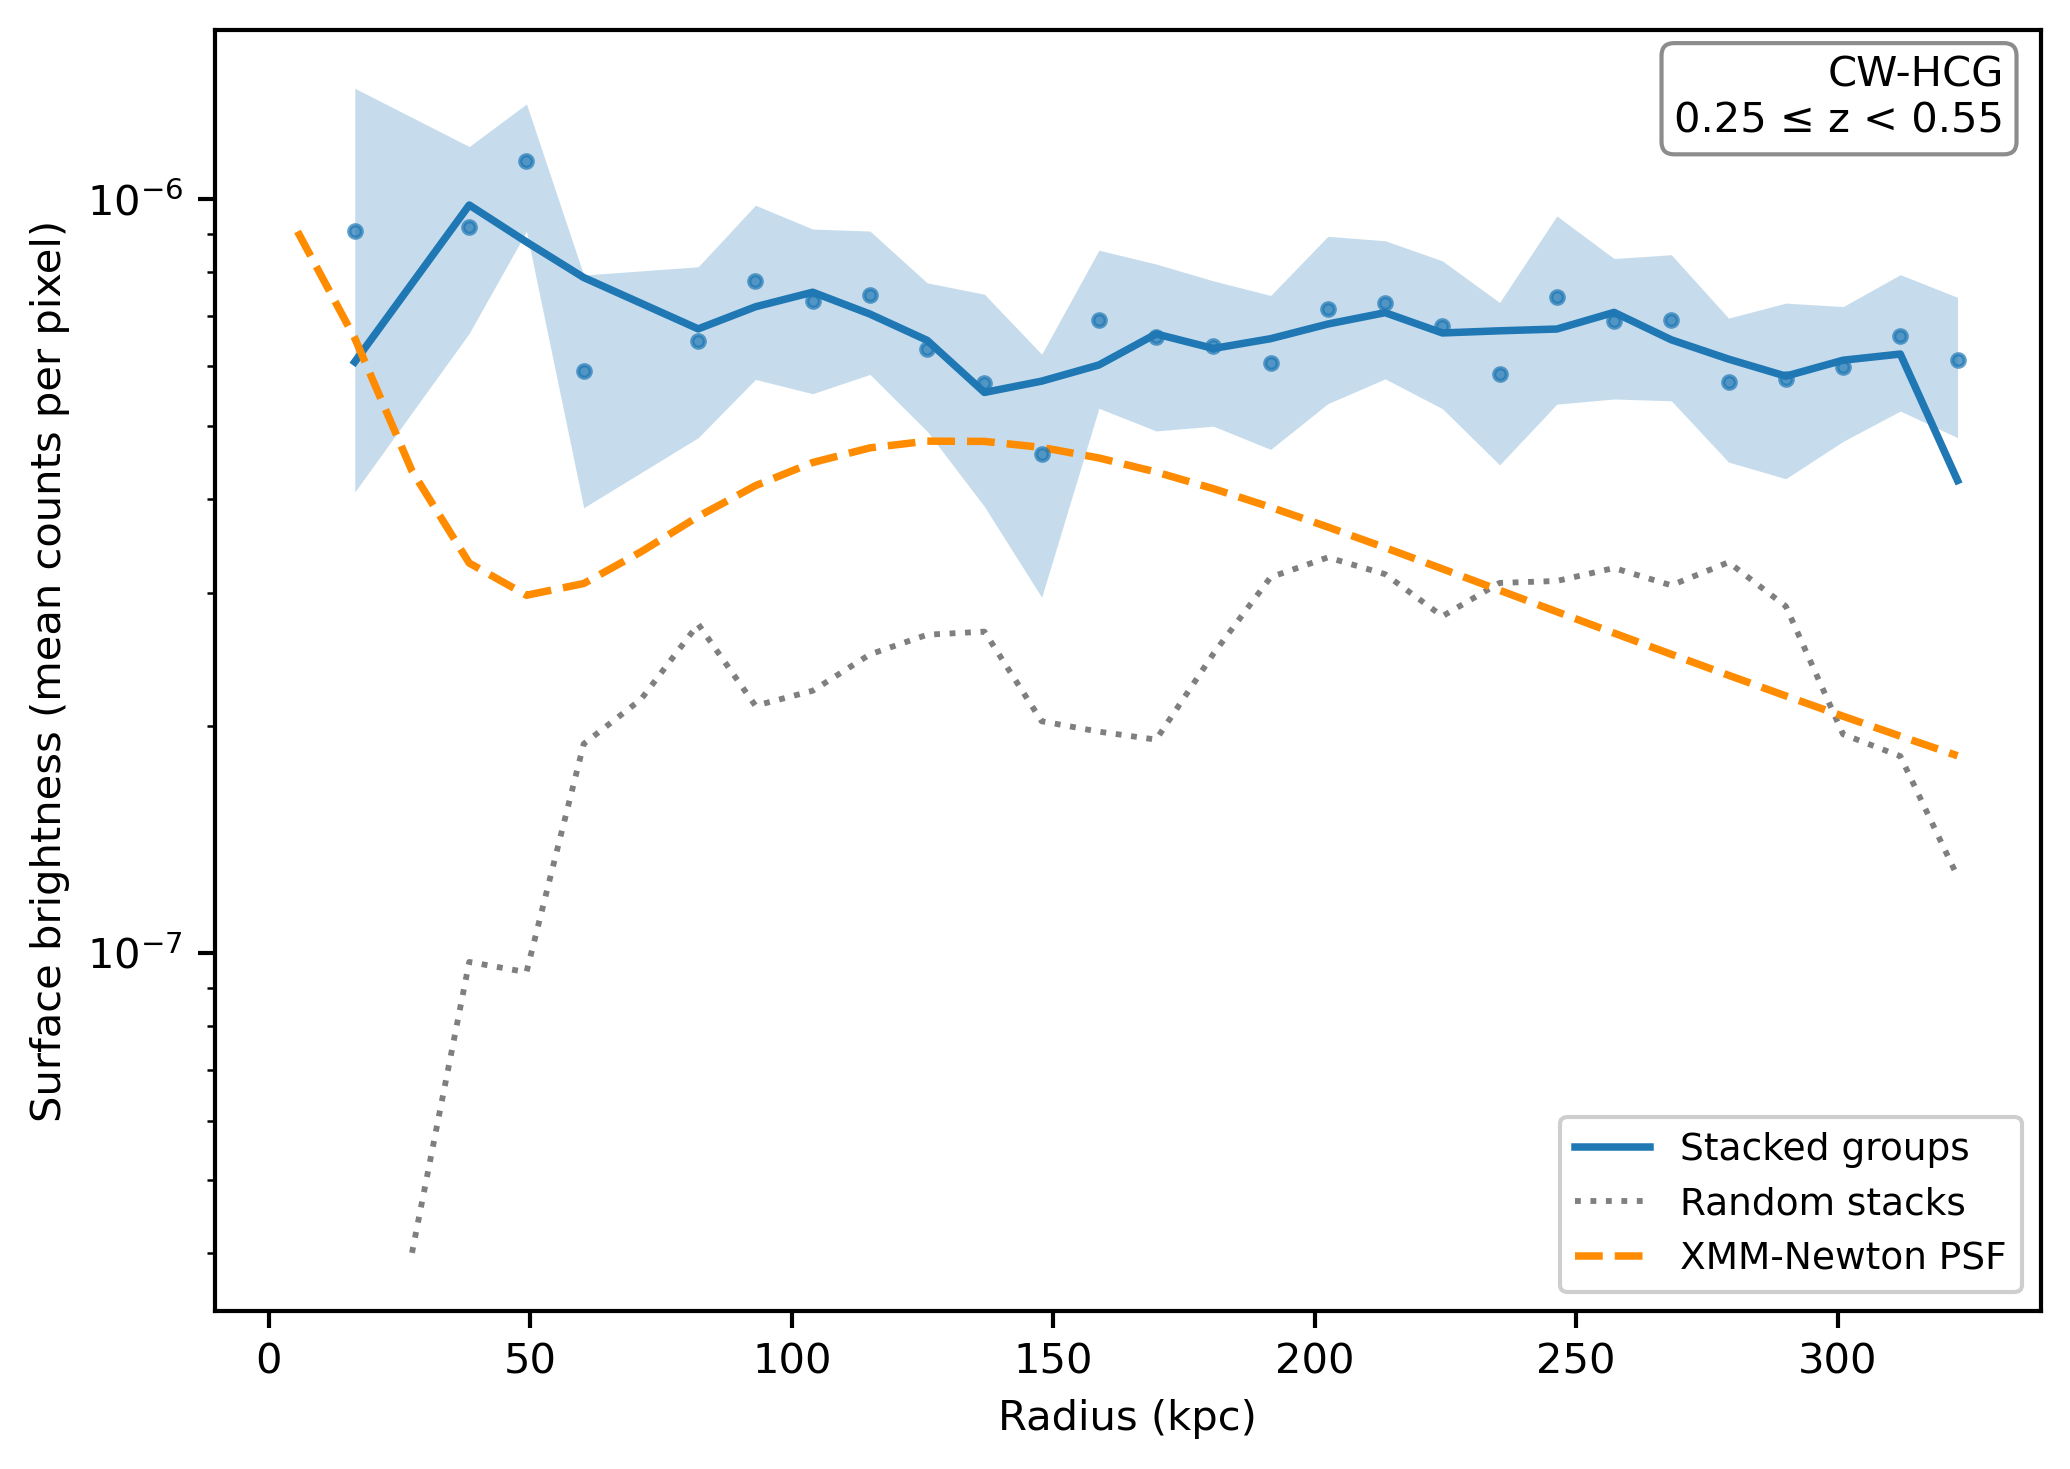
\includegraphics[width=0.32\textwidth]{figures/stacking_radial_profiles_z_0.25_0.55}
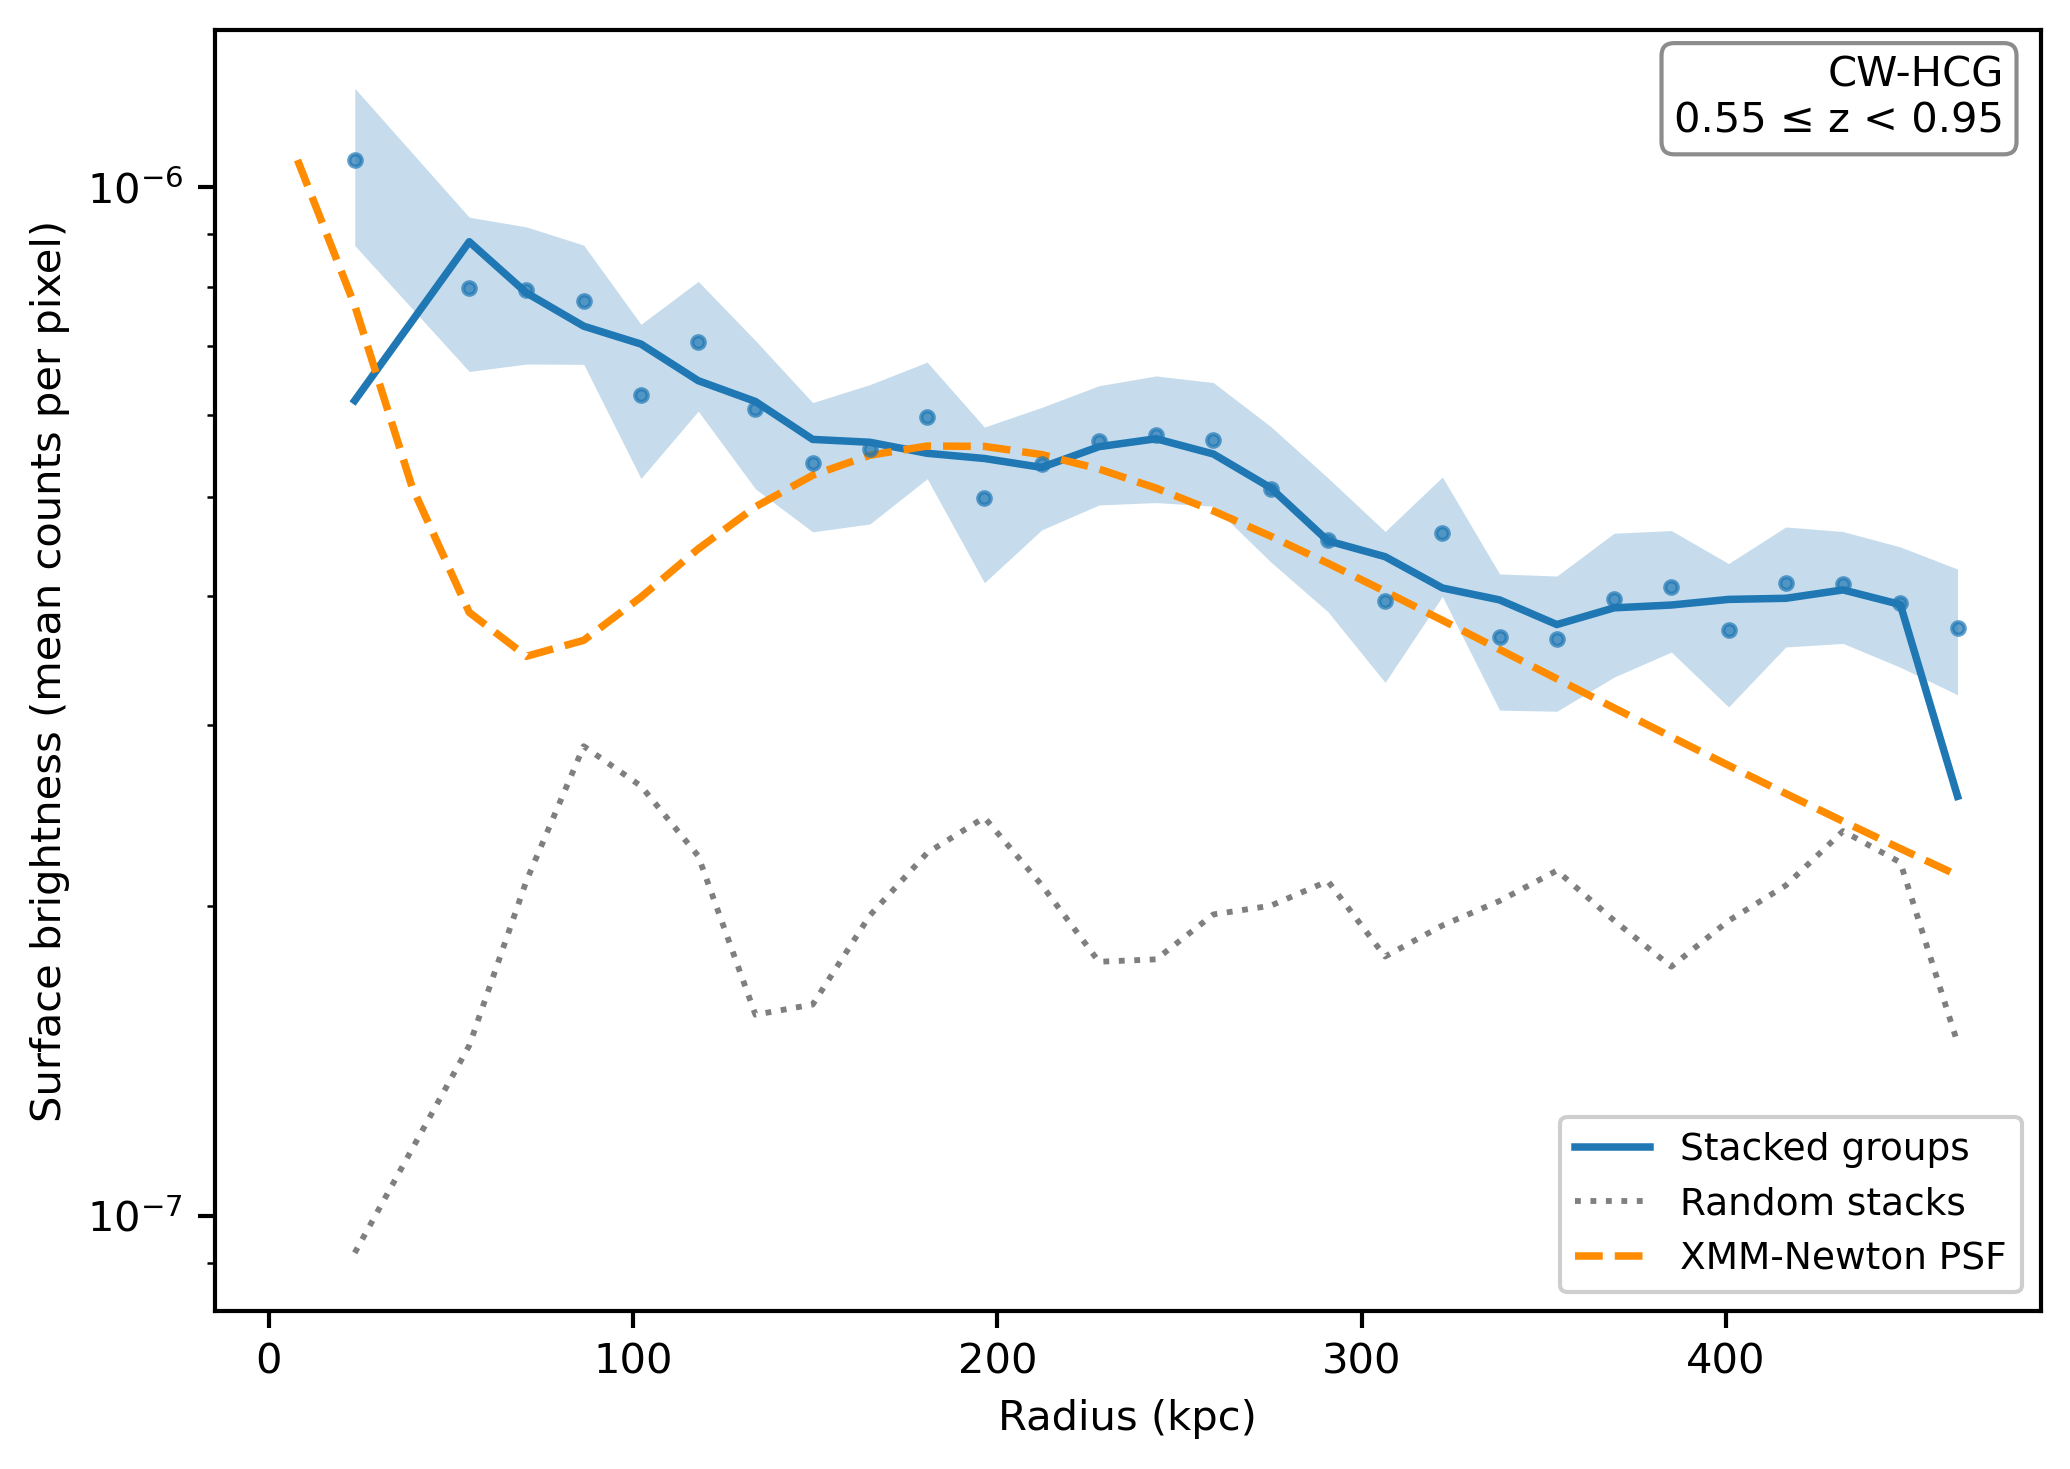
\includegraphics[width=0.32\textwidth]{figures/stacking_radial_profiles_z_0.55_0.95}
\caption{Same as Fig.~\ref{fig:profiles_all}, but for the compact-group subsample (CW-HCG). These panels highlight that compact systems are more centrally peaked and more significantly extended relative to the PSF at fixed redshift.}
\label{fig:profiles_hcg}
\end{figure*}

\begin{figure*}
\centering
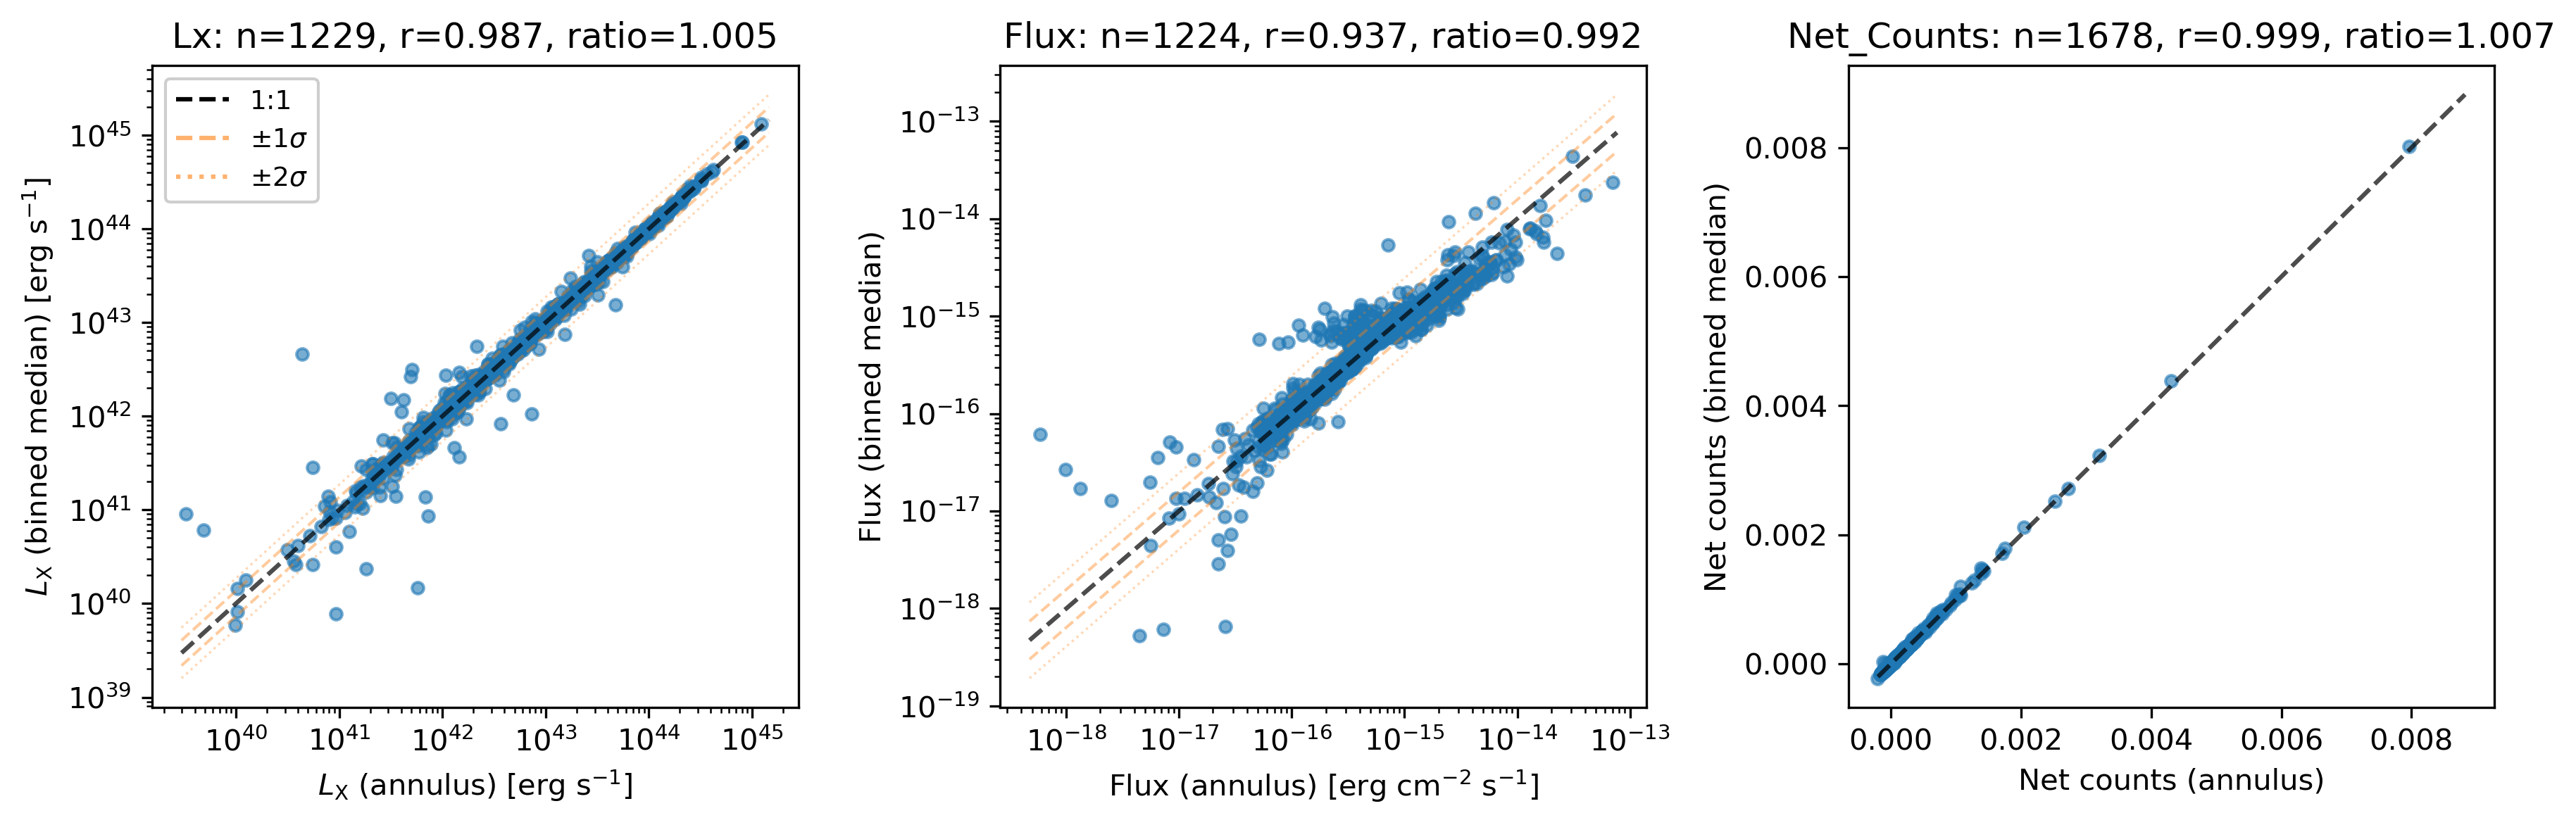
\includegraphics[width=\textwidth]{figures/background_comparison_photometry_cw_all}
\caption{Comparison of photometry obtained with annulus-based and redshift-binned median backgrounds for the CW-All sample. Panels show, from left to right, $L_{\rm X}$, flux, and net counts measured with annulus background (x-axis) versus binned-median background (y-axis). The black dashed line marks the 1:1 relation; orange bands indicate the $\pm1\sigma$ (solid) and $\pm2\sigma$ (dotted) scatter between the two methods in log space. The close clustering of points around the 1:1 line and near-unity median ratios demonstrate that the two background schemes are consistent and do not introduce significant systematic biases.}
\label{fig:background_comparison}
\end{figure*}

\end{document}
